%% ----------------------------------------
%%
%% NYU PhD thesis template.
%% Created by José Koiller 2007--2008.
%% Modified by Siddharth Krishna, 2019.

%%% ---------------Modified by Quynh M Nguyen, 2021.------------
%%  NYU Proquest Admin Approved. No Compilation error. Submittable to ArXiv. Bibliography with clickable DOI. 
%% to get DOI link added into a .bib file automatically, install a program in python bibtextparser
%%% https://tex.stackexchange.com/questions/6810/automatically-adding-doi-fields-to-a-hand-made-bibliography
%% ----------------------------------------


%% Use the first of the following lines during production to
%% easily spot "overfull boxes" in the output. Use the second
%% line for the final version.
%\documentclass[12pt,draft,letterpaper]{report}
\documentclass[12pt,oneside,letterpaper]{report}
%\DeclareUnicodeCharacter{0301}{*************************************}

% ----------------------------------------
% Macro to switch between draft version and final version
% ----------------------------------------

% Use or comment this to enable/disable draft version
% \def\draftversion{}
\newcommand{\draftfinal}[2]{\ifdefined\draftversion#1\else#2\fi}
\newcommand{\draftonly}[1]{\draftfinal{#1}{}}
\newcommand{\finalonly}[1]{\draftfinal{}{#1}}


% ----------------------------------------
% Thesis metadata
% ----------------------------------------

%% Replace the title, name, advisor name, graduation date and dedication below
%% with your own. Graduation months must be January, May or September.

% Adjust the space below the logo as needed
\newcommand{\thesistitle}{Quantum Random Number Generation Using the CQT Post Processor and CQT RNG Package: A Benchmarking and Explanatory Study}
\newcommand{\thesisauthor}{Ashraf Boussahi}
\newcommand{\thesisadvisor}{Dr. Taha Roubah}
\newcommand{\secondadvisor}{ {\color{black}{Mohamed Messaoud Louamri}}}


\newcommand{\thesisdept}{Physics}
\newcommand{\gradmonth}{January}
\newcommand{\gradyear}{2025}
%% If you do not want a dedication, scroll down and comment out
%% the appropriate lines in this file.
\newcommand{\thesisdedication}{To Albert Einstein...}


% ----------------------------------------
% Layout and formatting
% ----------------------------------------

% Uncomment to get a big black box to spot "overfull hboxes"
% \setlength{\overfullrule}{5pt}


%% Page layout (customized to letter paper and NYU requirements):
\RequirePackage[margin=1in, includefoot, letterpaper]{geometry}
\usepackage{pdfpages}

%% Color definitions:
\RequirePackage[prologue]{xcolor}
\definecolor[named]{ThesisBlue}{cmyk}{1,0.1,0,0.1}
\definecolor[named]{ThesisYellow}{cmyk}{0,0.16,1,0}
\definecolor[named]{ThesisOrange}{cmyk}{0,0.42,1,0.01}
\definecolor[named]{ThesisRed}{cmyk}{0,0.90,0.86,0}
\definecolor[named]{ThesisLightBlue}{cmyk}{0.49,0.01,0,0}
\definecolor[named]{ThesisGreen}{cmyk}{0.20,0,1,0.19}
\definecolor[named]{ThesisPurple}{cmyk}{0,94,95,0}
\definecolor[named]{ThesisDarkBlue}{cmyk}{1,0.58,0,0.21}

% School color found from university's graphic identity site:
% http://www.nyu.edu/employees/resources-and-services/media-and-communications/styleguide.html
\definecolor{SchoolColor}{cmyk}{0,0.94,0.95,0} % purple
\definecolor{chaptergrey}{rgb}{0.2600, 0.0200, 0.4600} % dialed back a little
\definecolor{midgrey}{rgb}{0.4, 0.4, 0.4}



%chemical formula
\usepackage{chemformula}
%table
\usepackage{array}

%% Captions of Figures, tables
\RequirePackage[labelfont={bf,sf,small,singlespacing},
                textfont={sf,small,singlespacing},
                % justification={justified,RaggedRight},
                % singlelinecheck=false,
                margin=0pt,
                figurewithin=chapter,
                tablewithin=chapter]{caption}

%% Chapter headings, captions
\usepackage{fix-cm}
\RequirePackage[raggedright,sc]{titlesec}
\definecolor{gray75}{gray}{0.75}
\newcommand{\hsp}{\hspace{20pt}}

\titleformat{\chapter}[hang]
{\Huge\sc}
{\textcolor{SchoolColor}{\thechapter}\hsp\textcolor{gray75}{|}\hsp}
{0pt}{\Huge\sc\raggedright}
% [\textcolor{gray75}{|}\hsp\textcolor{SchoolColor}{\thechapter}]


%% The following makes chapters and sections, but not subsections,
%% appear in the TOC (table of contents). Increase to 2 or 3 to
%% make subsections or subsubsections appear, respectively. It seems
%% to be usual to use the "1" setting, however.
\setcounter{tocdepth}{3}

%% Sectional units up to subsubsections are numbered. To number
%% subsections, but not subsubsections, decrease this counter to 2.
\setcounter{secnumdepth}{3}

%% Use the following commands, if desired, during production.
%% Comment them out for final version.
%\usepackage{layout} % defines the \layout command, see below
%\setlength{\hoffset}{-.75in} % creates a large right margin for notes and \showlabels

%% Controls spacing between lines (\doublespacing, \onehalfspacing, etc.):
\usepackage{setspace}

%% Use the line below for official NYU version, which requires
%% double line spacing. For all other uses, this is unnecessary,
%% so the line can be commented out.
\finalonly{
  \doublespacing % requires package setspace, invoked above
}

%% For generating sample text.
%% Can be removed when you've replaced all \lipsum commands with your text.
\usepackage{lipsum}
\usepackage{xcolor}
\usepackage{tcolorbox}

% ----------------------------------------
% Comments and TODOs:
% ----------------------------------------

% Uncomment this to remove all comments
\newcommand{\nocomments}{}

% Uncomment this to remove all TODOs
\newcommand{\notodos}{}

% Comments and TODOs
\newcommand{\fcomment}[2]{\ifdefined\nocomments{}\else\footnote{\textcolor{red}{#1:} #2}\fi}
\newcommand{\todo}[1]{\ifdefined\notodos{}\else\textcolor{red}{TODO\ifstrempty{#1}{}{: #1}}\fi}
\newcommand{\ftodo}[1]{\ifdefined\notodos{}\else\fcomment{TODO}{#1}\fi}

% Author comments:
\newcommand{\aen}[1]{\fcomment{Emmy}{#1}}


% ----------------------------------------
% User-specific packages and macros
% ----------------------------------------

%% This inputs your auxiliary file with \usepackage's and \newcommand's:
%% It is assumed that that file is called "defs.tex".
% ----------------------------------------
% Packages
% ----------------------------------------

% 
% Place here your \usepackage's. Some recommended packages are already included.
%

% Graphics:
%\usepackage[final]{graphicx}
\usepackage{graphicx} % use this line instead of the above to suppress graphics in draft copies
%\usepackage{graphpap} % \defines the \graphpaper command

% Uncomment this to indent first line of each section:
 \usepackage{indentfirst}

% Good AMS stuff:
\usepackage{amsthm} % facilities for theorem-like environments
%\usepackage[tbtags]{amsmath} % a lot of good stuff!

% Fonts and symbols:
\usepackage{amsfonts}
\usepackage{amssymb}

% Set the fonts
\RequirePackage[T1]{fontenc}
\ifxetex
  \RequirePackage[tt=false]{libertine}
\else
  \RequirePackage[tt=false, type1=true]{libertine}
\fi
\RequirePackage[varqu]{zi4}
\RequirePackage[libertine]{newtxmath}


% For typesetting inference rules
\usepackage{mathpartir}
% \usepackage{pftools}  % A local package
\newcommand{\bmmax}{2}
\usepackage{bm}

% Formatting tools:
%\usepackage{relsize} % relative font size selection, provides commands \textsmalle, \textlarger
%\usepackage{xspace} % gentle spacing in macros, such as \newcommand{\acims}{\textsc{acim}s\xspace}

% Page formatting utility:
%\usepackage{geometry}

\usepackage{booktabs}   %% For formal tables:
                        %% http://ctan.org/pkg/booktabs
\usepackage[labelformat=simple]{subcaption} %% For complex figures with subfigures/subcaptions
                        %% http://ctan.org/pkg/subcaption
% Options to subcaption are to label and refer to subfigures as Fig 1(a) etc.
\renewcommand\thesubfigure{(\alph{subfigure})}

\usepackage[T1]{fontenc} % needed for scaling fancy fonts (?)
\usepackage[utf8]{inputenc} % not sure this is needed

\usepackage{amssymb}
%\usepackage[table]{xcolor}

% For code
\usepackage[final]{listings}
\lstset{mathescape=true}

% For code highlighting
% \usepackage{bold-extra}

% Tikz
\usepackage{tikz}
\usetikzlibrary{matrix,arrows,positioning,calc,fit,backgrounds}

% To control enum item labelling/numbering
\usepackage[shortlabels, inline]{enumitem}
% To give custom item labels and reference them
\makeatletter
\newcommand{\myitem}[1][]{
  \protected@edef\@currentlabel{#1}%
\item[#1]
}
\makeatother

% To stop aligned env swallowing up []s
\usepackage{mathtools}

% To use ifstrempty
\usepackage{etoolbox}

% For math mode tables
\usepackage{array}
% A text column in array
\newcolumntype{L}{>$l<$}

% For \llbracket and \rrbracket
\usepackage{stmaryrd}

% For dashed boxes
\usepackage{dashbox}

% For big separating conjunction
\usepackage{scalerel}

% For mathpar environment
\usepackage{mathpartir}

\usepackage{xspace}
\usepackage{multirow}

% To stop citations overflowing lines
\usepackage{breakcites}

% For citet command
% \usepackage{natbib}
% \setcitestyle{%
%     authoryear,%
%     open={[},close={]},citesep={;},%
%     aysep={},yysep={,},%
%     notesep={, }}
% \let\cite\citep
%\usepackage[square,sort,comma,numbers]{natbib}

%%
%% Place here your \newtheorem's:
%%

\theoremstyle{plain}
\newtheorem{theorem}{Theorem}[chapter]
\newtheorem{conjecture}[theorem]{Conjecture}
\newtheorem{proposition}[theorem]{Proposition}
\newtheorem{lemma}[theorem]{Lemma}
\newtheorem{corollary}[theorem]{Corollary}
\theoremstyle{definition}
\newtheorem{example}[theorem]{Example}
\newtheorem{definition}[theorem]{Definition}
\theoremstyle{plain}


% ----------------------------------------
% Generic definitions
% ----------------------------------------
% Required packages: listings, tikz

% A footnote without a marker
\newcommand\blfootnote[1]{%
  \begingroup
  \renewcommand\thefootnote{}\footnote{#1}%
  \addtocounter{footnote}{-1}%
  \endgroup
}

\renewcommand{\le}{\leqslant}
\renewcommand{\ge}{\geqslant}
% \renewcommand{\emptyset}{\ensuremath{\varnothing}}
% \newcommand{\ds}{\displaystyle}

% Math stuff
\newcommand{\R}{\ensuremath{\mathbb{R}}}
\newcommand{\Q}{\ensuremath{\mathbb{Q}}}
\newcommand{\Z}{\ensuremath{\mathbb{Z}}}
\newcommand{\N}{\ensuremath{\mathbb{N}}}
\newcommand{\T}{\ensuremath{\mathbb{T}}}
\newcommand{\C}{\ensuremath{\mathbb{C}}}
\newcommand{\eps}{\varepsilon}
\newcommand{\closure}[1]{\ensuremath{\overline{#1}}}
%\newcommand{\acim}{\textsc{acim}\xspace}
%\newcommand{\acims}{\textsc{acim}s\xspace}

\newcommand{\Land}{\bigwedge}
\newcommand{\Lor}{\bigvee}
\newcommand{\es}{\emptyset}
\newcommand{\incl}{\subseteq}
\newcommand{\impl}{\Rightarrow}
\renewcommand{\iff}{\Leftrightarrow}
\newcommand{\ra}{\rightarrow}
\newcommand{\sat}{\vDash}
\newcommand{\notsat}{\nvDash}
\newcommand{\proves}{\vdash}
\newcommand{\provesIff}{\mathrel{\dashv\vdash}}
\newcommand{\boolTrue}{\top}
\newcommand{\boolFalse}{\bot}

\newcommand{\dom}{\operatorname{\mathsf{dom}}}
\newcommand{\range}{\operatorname{\mathsf{rng}}}
\newcommand{\restrict}[2]{{#1}|_{#2}}
\newcommand{\pto}{\rightharpoonup}

\newcommand{\defeq}{\coloneqq}
\newcommand{\defiff}{\vcentcolon\iff}

\newcommand{\pipe}{\triangleright}

%% Caligraphic
\newcommand{\Aa}{{\mathcal{A}}}
\newcommand{\Bb}{{\mathcal{B}}}
\newcommand{\Cc}{{\mathcal{C}}}
\newcommand{\Dd}{{\mathcal{D}}}
\newcommand{\Ee}{{\mathcal{E}}}
\newcommand{\Ff}{{\mathcal{F}}}
\newcommand{\Gg}{{\mathcal{G}}}
\newcommand{\Hh}{{\mathcal{H}}}
\newcommand{\Ii}{{\mathcal{I}}}
\newcommand{\Jj}{{\mathcal{J}}}
\newcommand{\Kk}{{\mathcal{K}}}
\newcommand{\Ll}{{\mathcal{L}}}
\newcommand{\Mm}{{\mathcal{M}}}
\newcommand{\Nn}{{\mathcal{N}}}
\newcommand{\Oo}{{\mathcal{O}}}
\newcommand{\Pp}{{\mathcal{P}}}
\newcommand{\Qq}{{\mathcal{Q}}}
\newcommand{\Rr}{{\mathcal{R}}}
\newcommand{\Ss}{{\mathcal{S}}}
\newcommand{\Tt}{{\mathcal{T}}}
\newcommand{\Uu}{{\mathcal{U}}}
\newcommand{\Vv}{{\mathcal{V}}}
\newcommand{\Ww}{{\mathcal{W}}}
\newcommand{\Yy}{{\mathcal{Y}}}
\newcommand{\Zz}{{\mathcal{Z}}}

% Wrappers: Parens, brackets, etc
% \newcommand{\op}[1]{\operatorname{#1}}
\newcommand{\paren} [1] {\ensuremath{ \left( {#1} \right) }}
\newcommand{\bigparen} [1] {\ensuremath{ \Big( {#1} \Big) }}
% \newcommand{\bracket}[1]{\left[#1\right]}
\newcommand{\tuple}[1]{\ensuremath{\langle #1 \rangle}}
\newcommand{\abs}[1]{\ensuremath{\lvert #1 \rvert}}
% \newcommand{\set}[1]{\ensuremath{\left\{#1\right\}}}
\newcommand{\setcomp}[2]{\ensuremath{\left\{#1\;\middle|\;#2\right\}}}

% References
\newcommand{\refCh}[1]{Chapter~\ref{#1}}
\newcommand{\refSc}[1]{Section~\ref{#1}}
% \newcommand{\refSc}[1]{\S\ref{#1}}
\newcommand{\refFig}[1]{Figure~\ref{#1}}
\newcommand{\refDef}[1]{Definition~\ref{#1}}
\newcommand{\refLem}[1]{Lemma~\ref{#1}}
\newcommand{\refThm}[1]{Theorem~\ref{#1}}
\newcommand{\refAlg}[1]{Algorithm~\ref{#1}}
\newcommand{\refEx}[1]{Example~\ref{#1}}
\newcommand{\refCor}[1]{Corollary~\ref{#1}}
\newcommand{\refTab}[1]{Table~\ref{#1}}
\newcommand{\refEq}[1]{\ensuremath{(\ref{#1})}}
\newcommand{\refRule}[1]{(\ref{#1})}
\newcommand{\refApp}[1]{Appendix~\ref{#1}}

\newcommand{\tool}[1]{\textsf{#1}}
\newcommand{\code}[1]{\textnormal{\small\texttt{#1}}}
% \newcommand{\code}[1]{\text{\lstinline{#1}}}

% TODO have macros for \forall and \exists

\newcommand{\tick}{\ensuremath{\checkmark}}
\newcommand{\cross}{\text{\sffamily X}}


% ----------------------------------------
% Paper specific macros & commands
% ----------------------------------------


% Put your definitions here


%%% Local Variables:
%%% mode: latex
%%% TeX-master: "thesis"
%%% End:



% ----------------------------------------
% Document header
% ----------------------------------------

%% Cross-referencing utilities. Use one or the other--whichever you prefer--
%% but comment out both lines for final version.
%\usepackage{showlabels}
%\usepackage{showkeys}

%\usepackage[utf8]{vietnam}
\usepackage{comment}

\usepackage{hyperref}
\hypersetup{colorlinks,
  linkcolor=ThesisDarkBlue,
  citecolor=ThesisPurple,
  urlcolor=ThesisDarkBlue,
  filecolor=ThesisDarkBlue}
 
\usepackage[
url=false, 
doi=true,
sorting=none
]{biblatex}
\addbibresource{thesis.bib}



 
 \usepackage{lscape}
 
\begin{document}
%% Produces a test "layout" page, for "debugging" purposes only.
%% Comment out for final version.
%\layout % requires package layout (see above, on this same file)


%%%%%% Title page %%%%%%%%%%%
%% Sets page numbering to "roman style" i, ii, iii, iv, etc:
\pagenumbering{roman}
%
%% No numbering in the title page:
\thispagestyle{empty}
%
%\begin{center}
%\includegraphics[scale=2]{nyu_stacked_color.jpg}    
%\end{center}

\vspace*{25pt}
\begin{center}
    
    % Add the logo at the top
    

  {\Large
    \begin{doublespace}
      {\textcolor{SchoolColor}{\textsc{\thesistitle}}}
    \end{doublespace}
  }
  \vspace{.7in}

  by
  \vspace{.7in}

  \thesisauthor
  \vfill

  \begin{doublespace}
    \textsc{
    A final report submitted in fulfillment\\
    of the requirements of\\
    the Internship at\\
    Constantine Quantum Technology \\
    \gradmonth, \gradyear}
  \end{doublespace}
\end{center}
\vfill

\noindent\makebox[\textwidth]{\hfill\makebox[2.5in]{\hrulefill}}\\
\makebox[\textwidth]{\hfill\makebox[2.5in]{\hfill\thesisadvisor}}
\noindent\makebox[\textwidth]{\hfill\makebox[2.5in]{\hrulefill}}\\
\makebox[\textwidth]{\hfill\makebox[2.5in]{\hfill\secondadvisor}}





%%%%%%%%%%%%%% Dedication %%%%%%%%%%%%%%%%%
%% Comment out the following lines if you do not want to dedicate
%% this to anyone...
%\cleardoublepage
%\phantomsection
%\chapter*{Dedication}
%\addcontentsline{toc}{chapter}{Dedication}
%\vspace*{\fill}
%\begin{center}
 % \thesisdedication
%\end{center}
%\vfill
%\newpage


%%%%%%%%%%%%%% Acknowledgements %%%%%%%%%%%%
%% Comment out the following lines if you do not want to acknowledge
%% anyone's help...
\chapter*{Acknowledgements}
\addcontentsline{toc}{chapter}{Acknowledgments}

I am grateful to Dr. Taha, the principal investigator of the Constantine Quantum Technology Group, for giving me the chance to work with his brilliant team in a field I truly adore and will certainly try to make others appreciate as well.

I thank my supervisor, Mohammed Messaoud Louamri, for his great support, kindness, and extensive knowledge.

I also express my gratitude to Bohr, Schrödinger, and Einstein for giving humanity this quantum science, which will undoubtedly conquer and become a major part of mankind's future.



%\newpage


%%%% Abstract %%%%%%%%%%%%%%%%%%
\chapter*{Abstract}
\addcontentsline{toc}{chapter}{Abstract}

This study aims to explore the concepts and proposed schemes to achieve True Random Number Generators (TRNGs), focusing on Entropy Sources where the characteristics of Quantum Systems provide excellent irreproducible randomness, yet with some defects that can be overcome using: The Post Processors. 
In this work, we introduce, explore, and benchmark a novel PostProcessing approach called CQTPP and some of its variants CQTPP+MarkovChain, highlighting its good performance in decorrelating and debiasing a biased and dependent input, at the cost of extraction efficiency, which we attempted to improve slightly through a proposed scheme called Itterative CQTPP. We also introduce the cqt\_rng package and how we tried to improve it and introduce some  novel parts, this library implements Quantum Random Number Generation based on Boson Sampling also revisited in this study.

\newpage


%%%% Table of Contents %%%%%%%%%%%%
\tableofcontents



%%%%% List of Figures %%%%%%%%%%%%%
%% Comment out the following two lines if your thesis does not
%% contain any figures. The list of figures contains only
%% those figures included within the "figure" environment.
\cleardoublepage
\phantomsection
\addcontentsline{toc}{chapter}{List of Figures}
\listoffigures
\newpage


%%%%% List of Tables %%%%%%%%%%%%%
%% Comment out the following two lines if your thesis does not
%% contain more than one table. The list of tables contains only
%% those tables included within the "table" environment.
%\cleardoublepage
%\phantomsection
%\addcontentsline{toc}{chapter}{List of Tables}
%\listoftables
%\newpage


%%%%% Body of thesis starts %%%%%%%%%%%%
\pagenumbering{arabic} % switches page numbering to arabic: 1, 2, 3, etc.


% ----------------------------------------
% Body of Thesis
% ----------------------------------------

%\chapter{Introduction}
%\label{chp-introduction}

%\chapter{Introduction}
%\input{chapters/1-intro}

\chapter{Introduction} \label{ch1}


Randomness can be referred to as the property that a set of information \textbf{cannot be certainly predicted}, where there is no defined and deterministic pattern in how they were sorted or generated. According to Kendall and Babington Smith \cite{489b709a-b56c-3c3f-bfcb-5d1507b7d20e}, it refers, in casual terms, to a method of choice that \textbf{lacks aim or purpose}. In terms of statistics, it takes on more specific definitions closely related to \textbf{probability}, focusing on the aspect of \textbf{statistical frequencies} within the random information and studying their \textbf{degree of uncertainty}, as well as \textbf{judging} whether any given data or sampling method is random or not.

This concept of randomness is the core of many fields, some of which reach a serious and sensitive level. While randomly generated numbers are used in game development and the lottery industry \cite{10.1007/978-981-15-4474-3_4}, there are some crucial uses of it, mainly in the security of information systems \cite{Shanon} and cryptography \cite{Crypto}, where it plays a pivotal role in generating and producing keys and digital signatures for communication protocols used in IoT (Internet of Things) devices to transfer personal and highly confidential materials.

These crucial and highly demanded usages require the random numbers to adhere to a high rate of randomness by assuring some of the main characteristics: \textbf{unpredictability, unreproducibility, and a uniform and equally probable distribution}. In order to achieve that, several schemes have been proposed, designing the structures of \textbf{Random Number Generators (RNGs)}.



\section{Random Number Generators (RNGs) \& True Random Number Generators (TRNGs)}
An \textbf{RNG} is a system that generates numbers with the essential property of unpredictability, using various techniques and algorithms. As a general concept, an RNG can take many forms, such as physical ones like a \textbf{dice}, a \textbf{game wheel}, a \textbf{Galton Board}, or integrated algorithms in a \textbf{classical computer}, or even a \textbf{quantum computer}.

In the previous section, we mentioned the three main features that help judge the randomness of a generated number. By ensuring all these properties in a generation system (automatically applicable to the sampled data), a random number can be referred to as a \textbf{True Random Number}, and its generator as a \textbf{True Random Number Generator (TRNG)}. These features are:

\begin{itemize}
    \item \textbf{Unpredictability}: In a sequence of truly generated random numbers, the next generated value cannot be guessed, and each generation is independent of the previous values. This means that the next value cannot be determined based on the previously generated values. \textbf{Note}: The absence of this feature collapses the randomness of the generator (the generator is not random).
    
    \item \textbf{Unreproducibility}: For large number sequences, true random number generation cannot be reproduced. As the length of the sequence increases, the likelihood of generating two identical sequences decreases and converges to zero.
    
    \item \textbf{Uniform Distribution}: After a long series of true random generations, all possible basic values that the generator could produce should appear with equal likelihood, with no bias toward any specific value. This also applies to their possible combinations, which should appear equiprobably. \\
    \textit{E.g.}: In a generated bitstream, the probability of bits being 0 and the probability of bits being 1 should be equal but also, the probability of the two-bit words (\textbf{00}, \textbf{01}, \textbf{10}, \textbf{11}) should also be equal and so on for all possible combinations.
\end{itemize}



\section{Pseudorandom Number Generators PRNGs}
Nowadays, most of the random numbers used in cryptographic algorithms to encode our sensitive online materials (bank accounts, passwords, data sharing, and network tokens) are generated using classical computers and complicated algorithms. It may sound strange, but for a classical computer, no matter how advanced it is, it is difficult to get a computer to do something by chance. A computer running a program follows its instructions blindly and is therefore completely predictable \cite{haahr1999random}.

These kinds of generators are called \textbf{Pseudo-Random Number Generators} (PRNGs). They use discrete algorithms and calculations starting from an initial number called the \textbf{Seed}, such as the \textbf{Linear Congruential Generator (LCG)} described in \cite{LCG}. This method uses the following formula:
\begin{equation}
X_{i+1} = (aX_i + c) \mod M
\end{equation}
where \( a \) is a multiplier relatively prime to \( M \), and \( c \) is an increment, both chosen \textbf{appropriately}. Then, starting at a random seed \( X_0 \), the sequence \( \{X_i\} \) is generated.

The method successfully passes several randomness tests, but it breaks through the principle of \textbf{Unreproducibility}. Knowing the value of the seed (if it is leaked or somehow stolen) will allow one to reproduce the exact same random numbers and predict the next ones. We show in Appendix One how the same seed would reproduce the exact same sequence, and how this could break the encryption methods. Thus, the generated numbers appear to be random, but they are not.

Several other advanced algorithms have been proposed in order to reduce these risks, like the \textbf{Mersenne Twister based on linear shift feedback registers} \cite{matsumoto_1998_mersenne}, and \textbf{One-Time Pad (OTP) encryption} \cite{OTP}. These achieve good likelihood of randomness, but the fact that they are reproducible reduces the scope of their use.


\section{Quantum Random Number Generators (QRNGs)}
 A lot of schemes have been presented to create a True Random Number Generator that outputs true random numbers within the three aforementioned characteristics. Since \textbf{deterministic calculations could never generate a true random number}, some of the proposed schemes exploit and utilize \textbf{the randomness in physical noise} by sampling and processing a \textbf{hardware source of entropy} outside the computer. This can vary from using simple sources, like little variations in somebody’s mouse movements \cite{mouse}, to more advanced physical entropy sources, such as radiation \cite{radiation}, stable random telegraph noise \cite{RTN}, and different schemes that use \textbf{the basic randomness property features of various quantum systems} like Boson Sampling-based generators \cite{shi_Twa3na}, photon counting generators \cite{photonic}, generators based on quantum vacuum fluctuations \cite{Vaccum}, and others introduced and explained in \cite{OtherQrngs}.

These proposed schemes use \textbf{the physical uncertainty} of the systems as \textbf{entropy sources}. The raw extracted data from these methods often \textbf{exhibit statistical defects}, yet it \textbf{remains random} and in order to correct these defects, \textbf{deterministic algorithms} are applied to the generated data from the physical entropy source. 

The use of these deterministic concepts \textbf{does not affect the true randomness} of the generator, since the randomness source itself is \textbf{unreproducible}, and the post-processor is simply a method of \textbf{correction and extraction of maximum possible true randomness}.


Quantum Random Number Generators uses the same scheme of Entropy source-Post processor as you can see in Fig. \ref{fig:quanta}. 

\begin{figure}
\centering
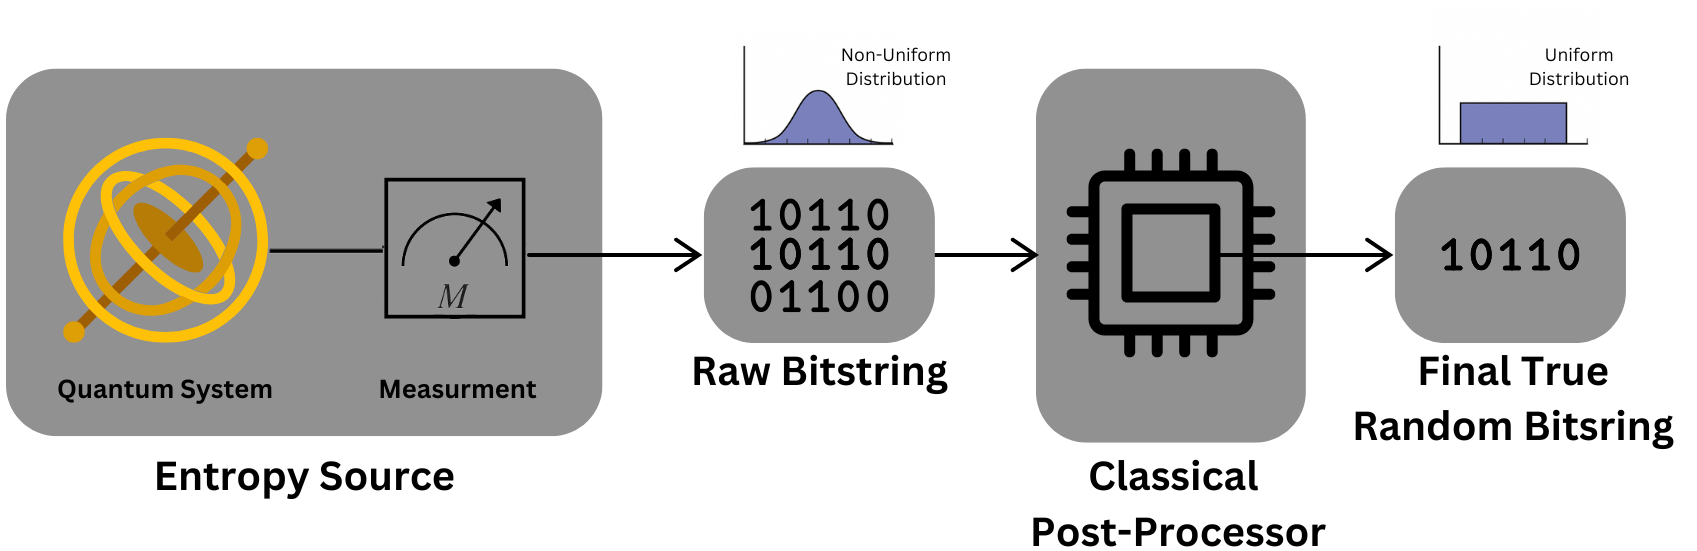
\includegraphics[width=16.5cm]{figures/Quantum System.png}\vspace{-0.2cm}
\caption{Quantum Random Number Generator (QRNG) Process}
\label{fig:quanta}
\end{figure}

\section{Post Processors (PP)}
\noindent
\begin{tcolorbox}[colframe=blue!20!white, colback=yellow!10!white, coltitle=black, title=Note]
     In this work, we will consider that Random Number Generators (RNGs) produce bitstrings, often referred to as \textit{bitstreams}, of length \(N\), where each atomic value can either be \(0\) or \(1\) \& We will model the systems and approaches based on this structure.
\end{tcolorbox}

In our context, \textbf{Post Processors (PP)} are \textbf{deterministic classical methods} applied to the \textbf{raw output} of an entropy source that generates random but \textbf{imperfect data}. These methods aim to \textbf{correct statistical defects} in the raw data to ensure that the final output meets true randomness standards. Several approaches have been proposed to address different types of defects observed in bitstreams. Below, we outline two main defects that post-processors aim to address: \textbf{Bias} and \textbf{Autocorrelation}.

\subsection{Bias}  
When examining the raw output of the entropy source, we can notice that the generated bitstream exhibits bias toward one of the atomic possible outcomes at various stages:  
- \textbf{1-bit bias:} The probability that a single bit is 0 (or 1) is higher than the probability that it is 1 (or 0, respectively).  
- \textbf{2-bit bias:} At the 2-bit stage, the probability that all the possible 2-bit patterns (00, 01, 10, 11) aren't equal.  
- \textbf{n-bit bias:} The probability that all the possible n-bit patterns aren't equal, which introduces bias at this level.

To quantify this property, we will use a mathematical measure of randomness: the Shannon Entropy.

\textbf{Shannon Entropy:}  
In our study, we will use a normalized version of the Shannon Entropy function to simplify the interpretation of the results:

\begin{equation}
H(A) = - \frac{1}{n} \sum_{i \in A_n} p_i \log_2 (p_i)
\end{equation}

Where:
\begin{itemize}
    \item \( A_n \) is the set of possible outcomes of \( n \) bits.
    \item \( p_i \) is the probability of the \( i \)-th outcome in \( A \).
    \item \( n \in \mathbb{N}, n \geq 1 \) is the number of bits or bit patterns we are analyzing; \( n \) can be greater than 2.  
    For example, if \( n=1 \), then \( A = \{ 0, 1 \} \); if \( n=2 \), then \( A = \{ 00, 01, 10, 11 \} \); and so on.
\end{itemize}

The value of \( H(A) \) ranges between 0 and 1. 
A value \textbf{close to 1} indicates \textbf{high randomness} (maximum entropy), meaning the bitstream is \textbf{unbiased} and \textbf{random}. Conversely, a value \textbf{close to 0} indicates \textbf{low randomness} (minimum entropy), meaning the bitstream is not random and biased.


\subsection{Autocorrelation (AC)}  
In a bitstream, AutoCorrelation (AC for short) measures the degree of \textbf{correlation} and \textbf{dependency} between the bits of \textbf{the same bitstream} at a \textbf{delay} (or \textbf{lag}) of \( k \).  
It indicates how likely it is that a bit at position \( i \) \textbf{will influence the nature of another bit} at position \( i+k \).

In our study, we are going to quantify the autocorrelation using the autocorrelation coefficients \( \phi_k \).

\textbf{Autocorrelation Coefficient Formula:}  
The autocorrelation coefficient at lag \( k \), denoted as \( \phi_k \), is calculated using the following formula:


\begin{equation}
\phi_k = \frac{\text{Cov}(X_i, X_{i+k})}{\sigma_X^2} = \frac{\sum_{i=1}^{i = n - k}[(X_i - \mu)(X_{i+k} - \mu)]}{\sum (X_i - \mu)^2}
\end{equation}

Where:
\begin{itemize}
    \item \( X_i \) represents the value of the bitstream at position \( i \), and \( X_{i+1} \) represents the value of the bitstream at position \( i+1 \)
    \item \( \text{Cov}(X_t, X_{t+k}) \) is the covariance between the bits at positions \( t \) and \( t+k \).
    \item \( \mu \) is the mean of the bitstream.
    \item \( \sigma_X^2 \) is the variance of the bitstream.
\end{itemize}

For \( k=1 \), the autocorrelation coefficient can also be calculated using \textbf{Pearson’s formula}:

\begin{equation}
\phi_1 = \frac{p_{11} p_{00} - p_{10} p_{01}}{p_1 p_0}
\end{equation}

Where:
\begin{itemize}
    \item \( p_{11}, p_{00}, p_{10}, p_{01} \) denote the probabilities (or frequencies) of each 2-bit pattern occurring in the bitstream.
    \item \( p_1 \) and \( p_0 \) are the probabilities of individual bits being 1 or 0, respectively.
\end{itemize}

The autocorrelation coefficient \( \phi_k \) takes values between -1 and 1 for any lag \( k \):
\begin{itemize}
    \item \( \phi_0 = 1 \): The autocorrelation at lag 0 is always 1 because a bit is always identical to itself.
    \item \textbf{Positive Autocorrelation} (\( \phi_k > 0 \)): The bits at positions \( i \) and \( i+k \) tend to be similar. For example, if the \( i \)-th bit is 0, the \( (i+k) \)-th bit is more likely to be 0 as well.
    \item \textbf{Negative Autocorrelation} (\( \phi_k < 0 \)): The bits at positions \( i \) and \( i+k \) tend to alternate. For example, if the \( i \)-th bit is 0, the \( (i+k) \)-th bit is more likely to be 1, and vice versa.
    \item \( \phi_k \) approaching 0 indicates that the bitstream becomes decorrelated for that lag, reflecting higher randomness and independence.
\end{itemize}

\textit{\textbf{Note: Implementation of the quantifying functions (Entropy and Autocorrelation) using Python is included in the Appendices.} }

 
In order to overcome the above shortcomings, several post-processing approaches were proposed. Alongside the aforementioned metrics, we also introduce the \textbf{Extraction Efficiency} Metric (ExE for short), which evaluates the \textbf{output bitstream length} of the Post Processor over the \textbf{input bitstream length} (the raw one we obtained from the \textbf{entropy source}). Its formula can be written as:

\begin{equation}
    \text{ExE} = \frac{\text{len}(Output)}{\text{len}(Input)}
\end{equation}

Based on this, and as mentioned in the work of Zhang et al. in \cite{dede}, we can distinguish 3 types of postprocessors:

\begin{itemize}
    \item \( \text{ExE} < 1 \) => (Output size \textbf{is less} than the input size), such as the simplest XOR function and the most common method: the Von Neumann method, introduced by John von Neumann in 1951 in \cite{von_1951_various}.
    \item \( \text{ExE} = 1 \) => (Output size \textbf{is the same} as the input size), such as Linear Feedback Shift Registers (LFSR) \cite{LSFR} and Markov Chains \cite{markov}.
    \item \( \text{ExE} > 1 \) => (Output size \textbf{is greater} than input size), such as the middle square method \cite{MSMeth}
\end{itemize}

Each of the above-mentioned methods can achieve different results in terms of bias and autocorrelation.

\textbf{\textit{Note: The implementation of the ExE function in python is included in the Appendecies}}

\noindent Let us examine the ones we will need later in this study:

\subsection{The Von Neuman PP}

The Von Neumann post-processing method \cite{von_1951_various} relies on \textbf{discarding some information} from the bitstring generated by the entropy source to construct a \textbf{new unbiased one}.

The method relies simply on devising the given bitstrings into pairs of \textbf{2 bits} and than apply the following mapping:

\begin{equation}
    \quad 00 \rightarrow \Lambda , \quad 01 \rightarrow 0 , \quad 10 \rightarrow 1 , \quad 11 \rightarrow \Lambda
\end{equation}

where \( \Lambda \) represents no output digit, so by discarding the pairs that contains similar bits which produces the biasdness in the results we can achieve better results.

The highest output rate that can be achieved using the Von Neumann Post Processor (PP) is limited to 25\% of the input rate (ExE = 0.25), and it decreases with the input bias \cite{zonga}.

Several \textbf{variations} with improvements to the original method's throughput have been introduced, such as the N-bits Von Neumann procedure proposed by Peter Elias \cite{peter}. While using \textbf{4 bits}, it achieved an output rate of 40.6\%, and with \textbf{8 bits and a waiting strategy}, it reached a 62.5\% output rate \cite{zonga}. Another variation is the Iterating Von Neumann method proposed by Yuval Peres \cite{yuval}. Each of these methods aims to increase the rate of the Von Neumann post-processor while preserving the unbiasedness of the output.

The Von Neumann Post Processing technique is well known for its ability to achieve zero bias with a minimum entropy guarantee, but at the cost of throughput. Additionally, the input must be independent and uniformly biased (the bias is fixed), and this method, along with its variants, cannot solve or reduce the autocorrelation in the input. \cite{dede}.

\textbf{\textit{Note: The implementation of the Classical Von Neumann function in python is included in the Appendecies}}

\subsection{The Markov Chain PP}  
Discrete-Time Markov chains help determine \textbf{the next state} of a system based on the knowledge of \textbf{the previous one}. This Markov model can be constructed by having \textbf{a finite space} of states (in our case, the number of states is the number of possible combinations according to \( M \), the size (length) of a single state that a Markov chain can work through, which is \( 2^M \)), a \textbf{transition probability matrix} that indicates the probabilities of moving from one state to another, and \textbf{an initial state} from which we can sample the next ones.  

Following this model, we can \textbf{generate an autocorrelated bitstring} with a defined autocorrelation coefficient.  

As an example, consider a Markov chain for \( M=1 \), where the possible states are 0 and 1. We denote the transition probabilities by \( T_{ij} \), where \( i \) represents the previous state and \( j \) the next state. For instance, \( T_{01} \) denotes the probability that the next bit is 1 if the previous one is 0, and so on.  

We can gather the transition probabilities into a transition matrix:  
\begin{equation}
TransitionMatrix = 
\left[\begin{array}{cc}
T_{00} & T_{01} \\
T_{10} & T_{11} 
\end{array}\right]
\end{equation}

\noindentThese transition probabilities follow the constraints: \( T_{00} + T_{01} = 1 \) and \( T_{10} + T_{11} = 1 \).  

\noindent The described scheme is illustrated in Fig. \ref{fig:MKV1}. 

\newline


Probabilities of each bit in a generated bitstring that follows the proposed model will be:

\begin{equation}
[P_0, P_1] = \left[ \frac{T_{01}}{1 + T_{01} - T_{11}}, 1 - \frac{T_{01}}{1 + T_{01} - T_{11}} \right]
\end{equation}

So:

\begin{equation}
P_1 = \frac{T_{01}}{1 + T_{01} - T_{11}}, \quad P_0 = 1 - P_1
\end{equation}

And:

\begin{equation}
\phi_1 = T_{11} - T_{01}, \quad \phi_k = (T_{11} - T_{01})^k = \phi_1^k
\end{equation}

with \( k \) being the lag of the autocorrelation function.

For more proof and explanation, check \cite{dede}.

\begin{figure}[h]
    \centering
    \begin{minipage}{0.45\textwidth}
        \centering
        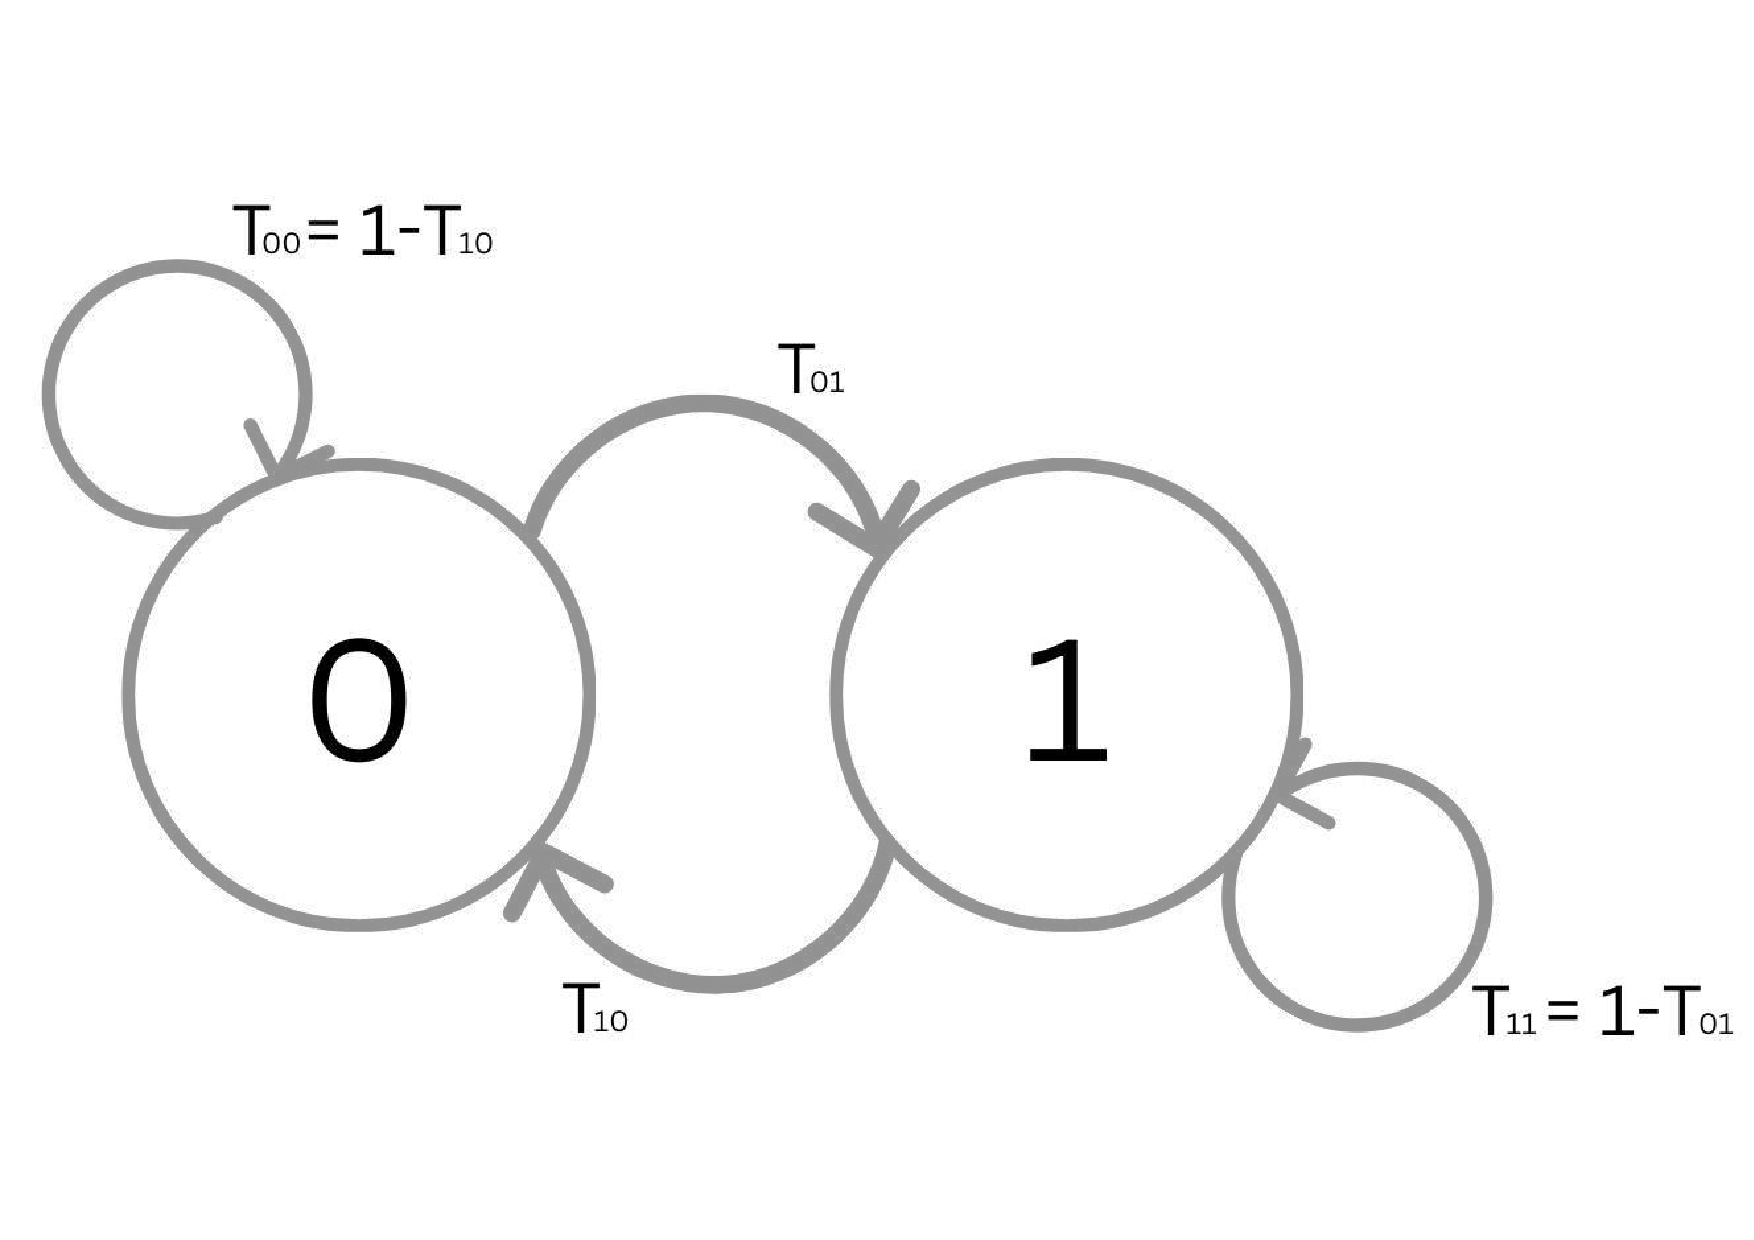
\includegraphics[width=\textwidth]{figures/MKV1.pdf}
        \caption{Diagram of Markov Chain with states of 1-bit}
        \label{fig:MKV1}
    \end{minipage}
    \hfill
    \begin{minipage}{0.45\textwidth}
        \centering
        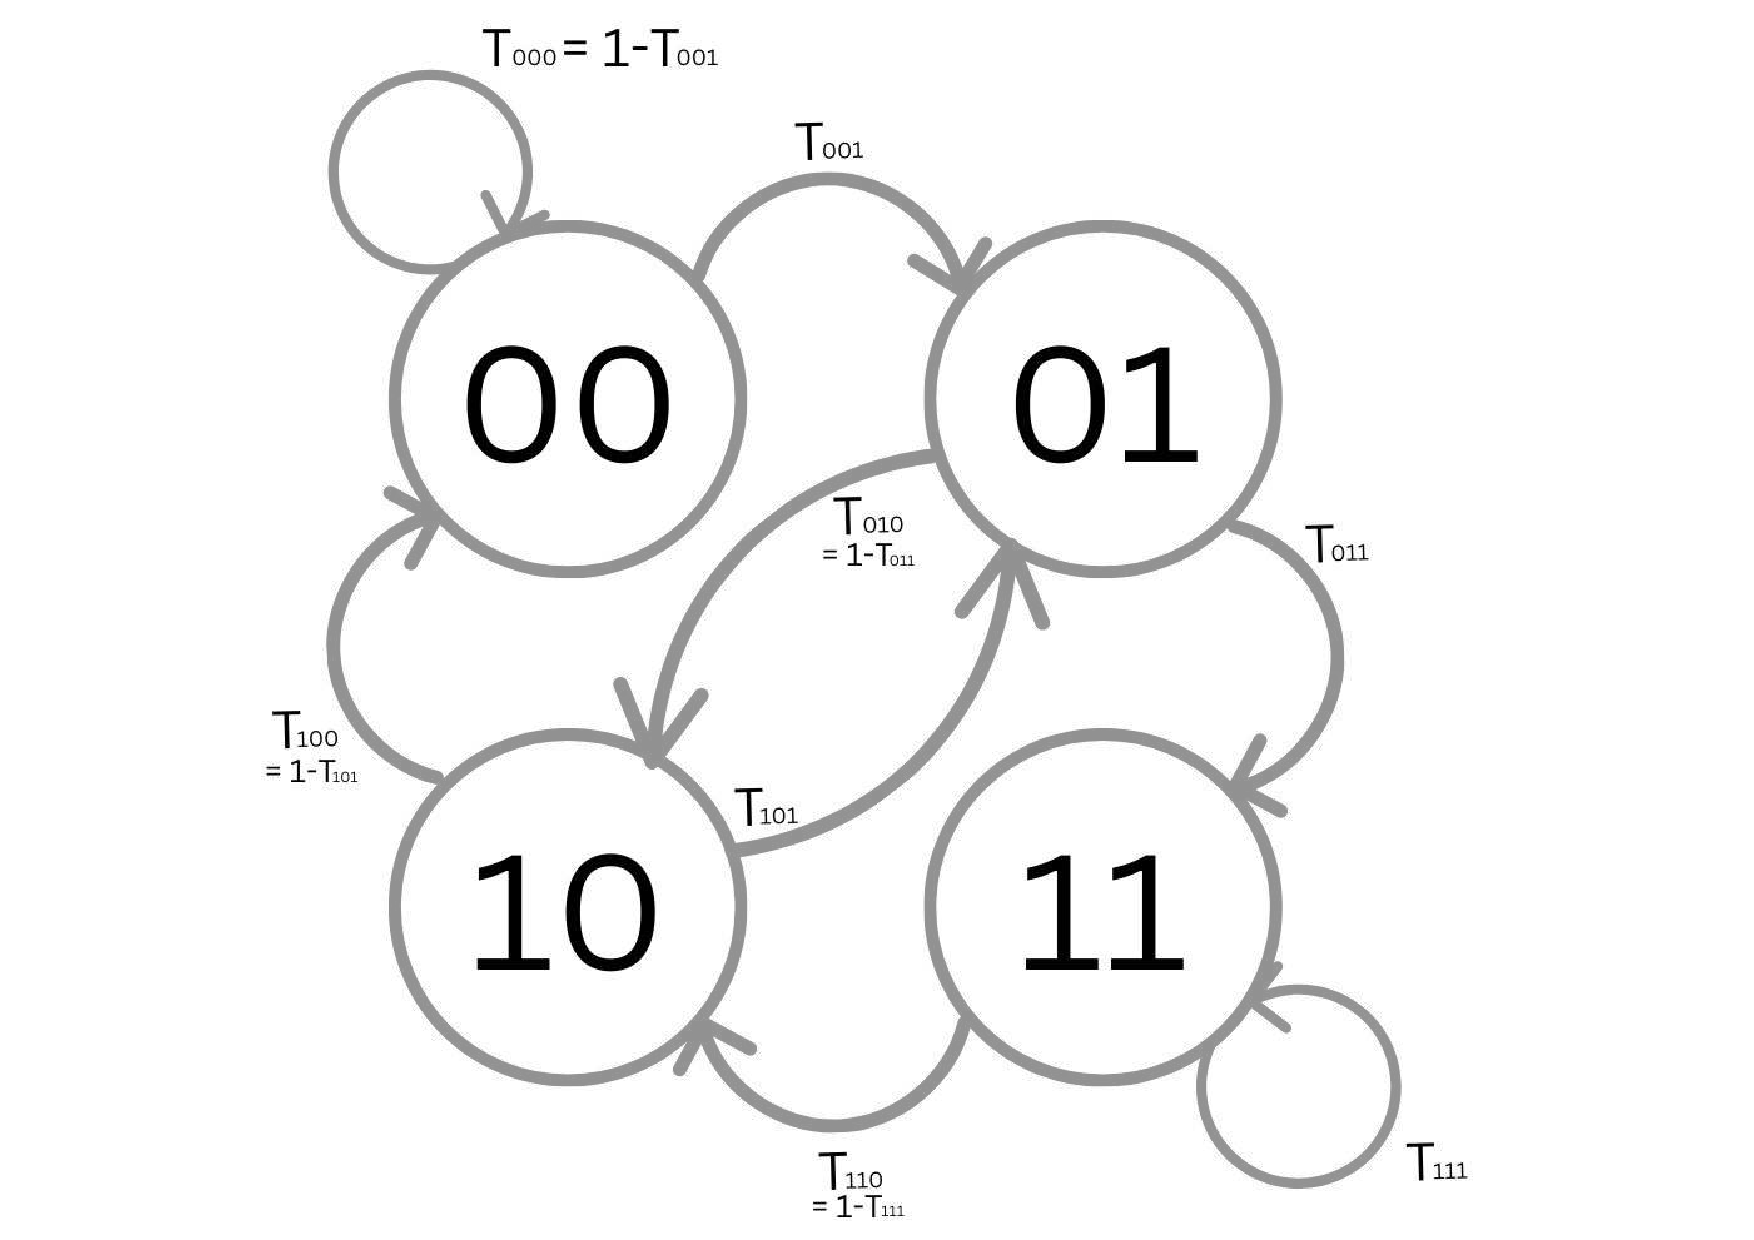
\includegraphics[width=\textwidth]{figures/MKV2.pdf}
        \caption{Diagram of Markov Chain with states of 2-bit}
        \label{fig:MKV2}
    \end{minipage}
\end{figure}

If we increase \( M \) to 2, we can have the 2-bit Markov chain model that has four states, and it is illustrated in Fig. \ref{fig:MKV2}.


Transition probabilities are denoted with \( T_{ijk} \), where the two states of 2 bits are \( ij \) and \( jk \), with \( j \) being an overlapped bit. For example, \( T_{010} \) is the probability of transition from state \( 01 \) to \( 10 \).

The post-processing technique that uses the above-mentioned principle of Markov chains to remove or reduce the correlation in the input can be achieved through \textbf{inverting the operation that generates the bitstring}, where \( M \) now represents the history size.

\begin{figure}[h]
    \centering
    \begin{minipage}{0.45\textwidth}
        \centering
        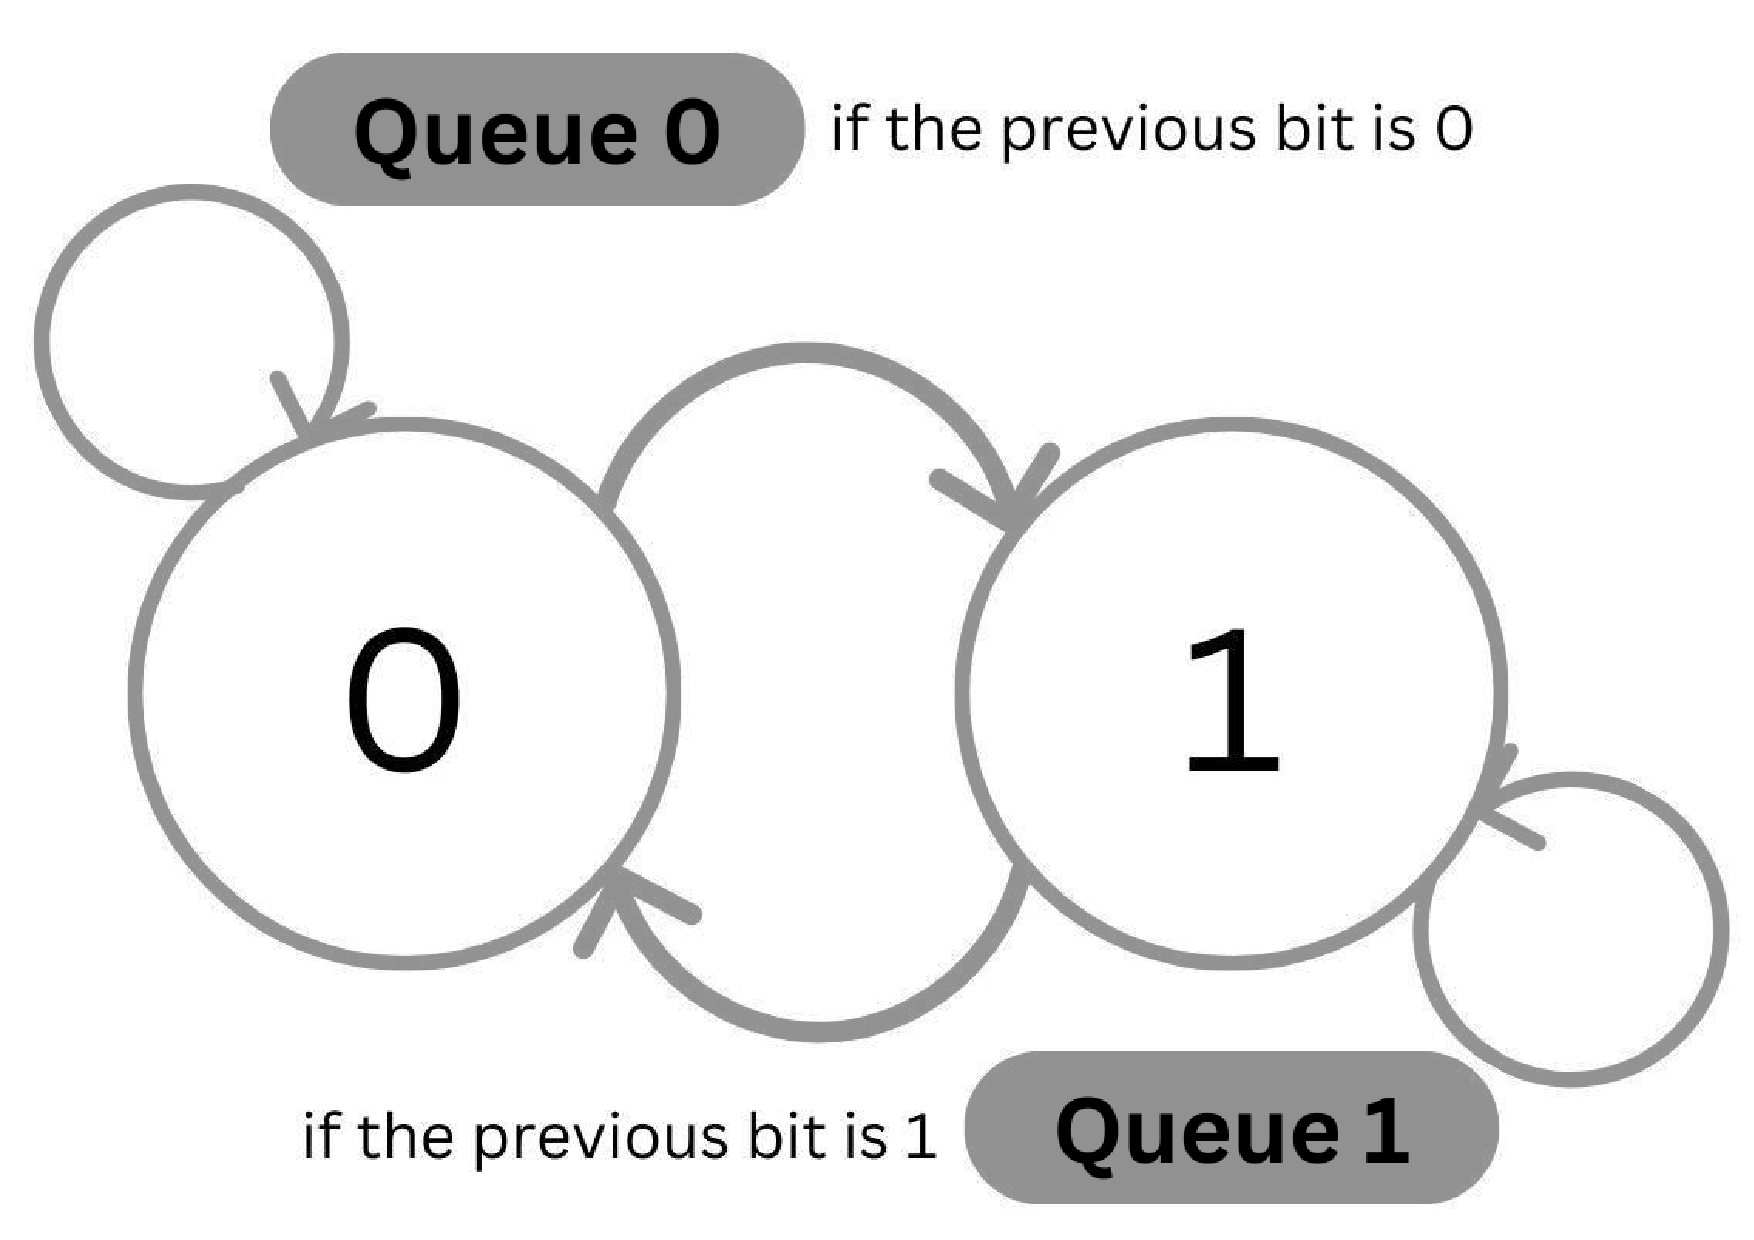
\includegraphics[width=\textwidth]{figures/mkv1 model.pdf}
        \caption{Diagram of Markov Chain de-correlation with 1-bit history}
        \label{fig:MKV22}
    \end{minipage}
    \hfill
    \centering
    \begin{minipage}{0.45\textwidth}
        \centering
        \includegraphics[width=\textwidth]{figures/MKV2_MODEL.pdf}
        \caption{Diagram of Markov Chain with states of 2-bit}
        \label{fig:MKV2mod}
    \end{minipage}
    
\end{figure}

The correlated input bitstream is routed using a Markov chain with \( M \)-bit history to \( 2^M \) queues:

For instance, \( M=1 \):  
The first bit is directly routed to the output.  
Starting from the second bit, if the previous one is 0, the bit is saved in \( \text{Queue}_0 \), and if it is 1, the bit is saved in \( \text{Queue}_1 \).  
At the end, we concatenate the two decorrelated queues (the order is not important).  
We can see the Markov de-correlation model in Fig. \ref{fig:MKV22}.


The entire process of the post-processor is illustrated in Fig. \ref{fig:MKVpp2}.

\begin{figure}
\centering
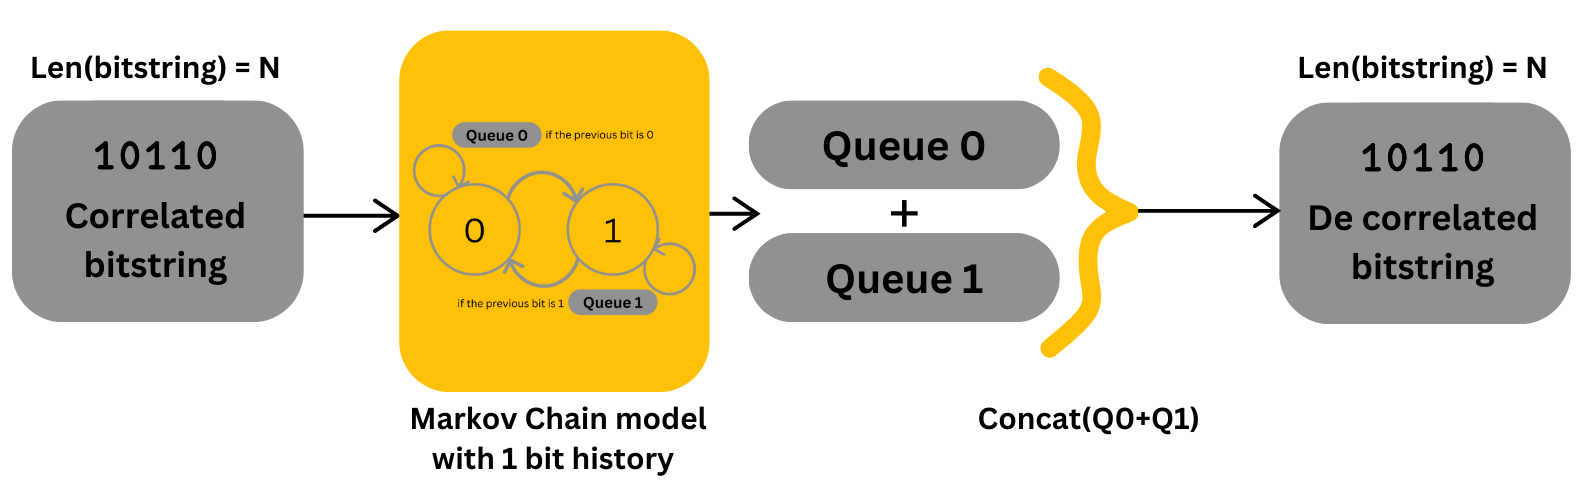
\includegraphics[width=16cm]{figures/De-Cor.png}\vspace{-0.2cm}
\caption{Post-Processing Method process using Markov Chain with 1-bit history and 2 queues}
\label{fig:MKVpp2}
\end{figure}



For instance, \( M=2 \):  
The first two bits are directly routed to the output.  
Starting from the third bit, if the previous two bits are \( 00 \), the bit is saved in \( \text{Queue}_{00} \), and so on.  
At the end, we concatenate the four decorrelated queues (the order is not important).  
We can see the Markov de-correlation model in Fig. \ref{fig:MKV2mod}.



The entire process of the post-processor that uses 2-bits history is illustrated in Fig. \ref{fig:MKV2dd}. 


\begin{figure}
\centering
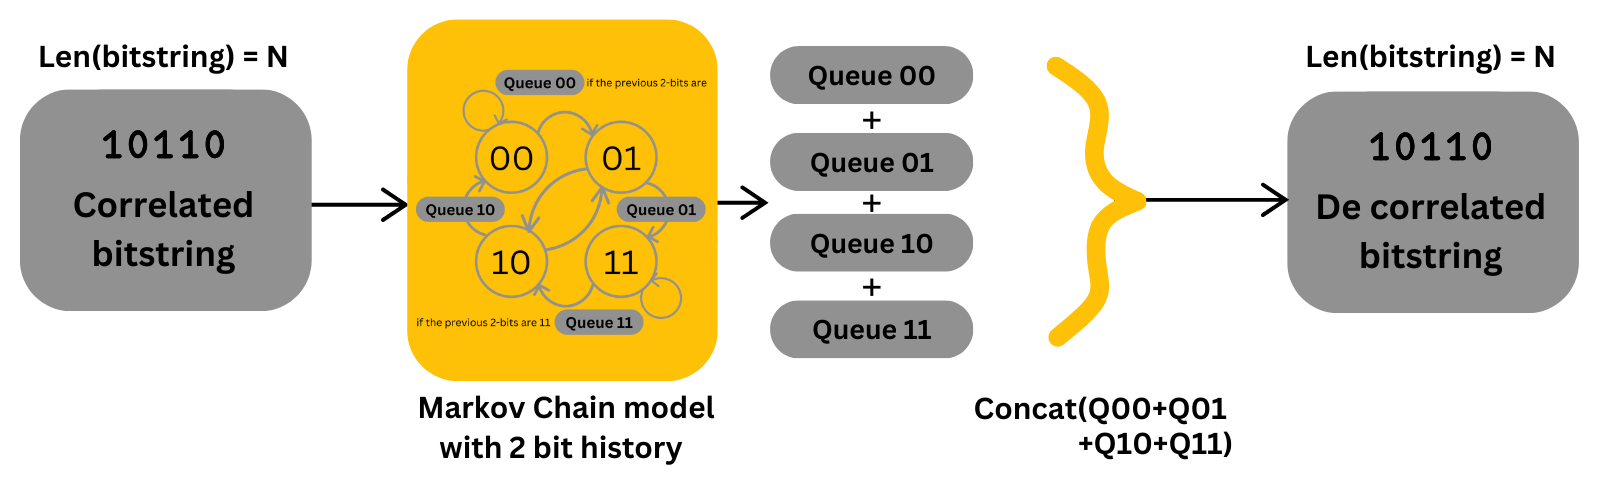
\includegraphics[width=16cm]{figures/De-Cor 2.png}\vspace{-0.2cm}
\caption{Post-Processing Method process using Markov Chain with 2-bits history and 4 queues}
\label{fig:MKV2dd}
\end{figure}

This scheme scores well in reducing the autocorrelation from the input, but since it discarded no bits, and the same length and bits are preserved, the bias of the bitstring and its entropy will not be improved.

A method to combine the properties of de-biasing from the Von Neumann PP and de-correlation from the Markov Chain PP was proposed by Zhang et al. in \cite{dede}, where the results were promising for different Markov models and randomly generated bitstrings, successfully passing most of the randomness tests, The diagram of the proposed flow is illustrated in Fig. \ref{fig:zhang}

\textbf{\textit{Note: The implementation of the Markov Model Bitstring Generation, and Markov Chain De-Correlation and Post Processing functions in python are included in the Appendecies}}


\begin{figure}
\centering
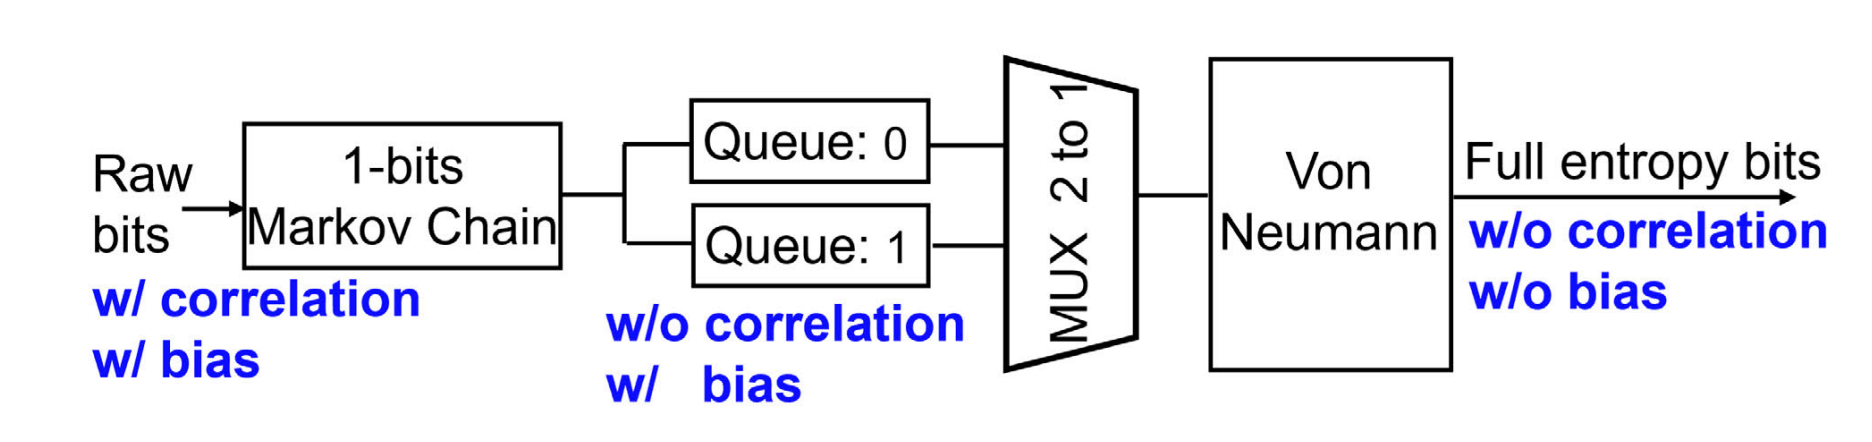
\includegraphics[width=16cm]{figures/ZHANG.png}\vspace{-0.2cm}
\caption{Diagram of de-correlation and de-bias by Markov chain and von
Neumann post-processing proposed by Zhang et Al in \cite{dede}}
\label{fig:zhang}
\end{figure}

\section{The Purpose And Goal of this Work \& Study}
In the previous subsections, we revisited the core principles surrounding True Random Number Generators (TRNGs) and explored various methods to improve the random but defective and imperfect output generated by physical entropy sources. We also listed the shortcomings of these methods.

The primary purpose of this study is to introduce and analyze a new post-processing method, hereby called the CQT Post Processor (CQTPP), along with its variants. This method aims to overcome the Von Neumann method's inability to handle dependent (autocorrelated) bitstreams. Additionally, we benchmark its results against other post-processing techniques using different hyperparameters to evaluate its performance in extracting true randomness from quantum entropy sources.

Special attention will be given to the Boson Sampling as an entropy source introduced in \cite{shi_Twa3na}, whose features in terms of randomness and sampling applications will be explored. Finally, we introduce a Python package, named CQT\_RNG, which integrates all these properties, methods, and metrics that were and will be discussed in this work
 








\chapter{Quantum Entropy Source using Boson Sampling} \label{ch2}
In their work \cite{boson}, Aaronson and Arkhipov introduced a quantum computation model in which a number of identical photons (which are considered boson particles) pass through a \textbf{linear optical network} and are then counted at the end of the network using photonic detectors, as shown in Fig. \ref{fig:bosonsample}. They provide evidence that computations relying on optical quantum elements cannot be efficiently simulated by classical computers. This feature makes it a good foundation to create a True Random Number Generator using this model as an entropy source.

\begin{figure}
\centering
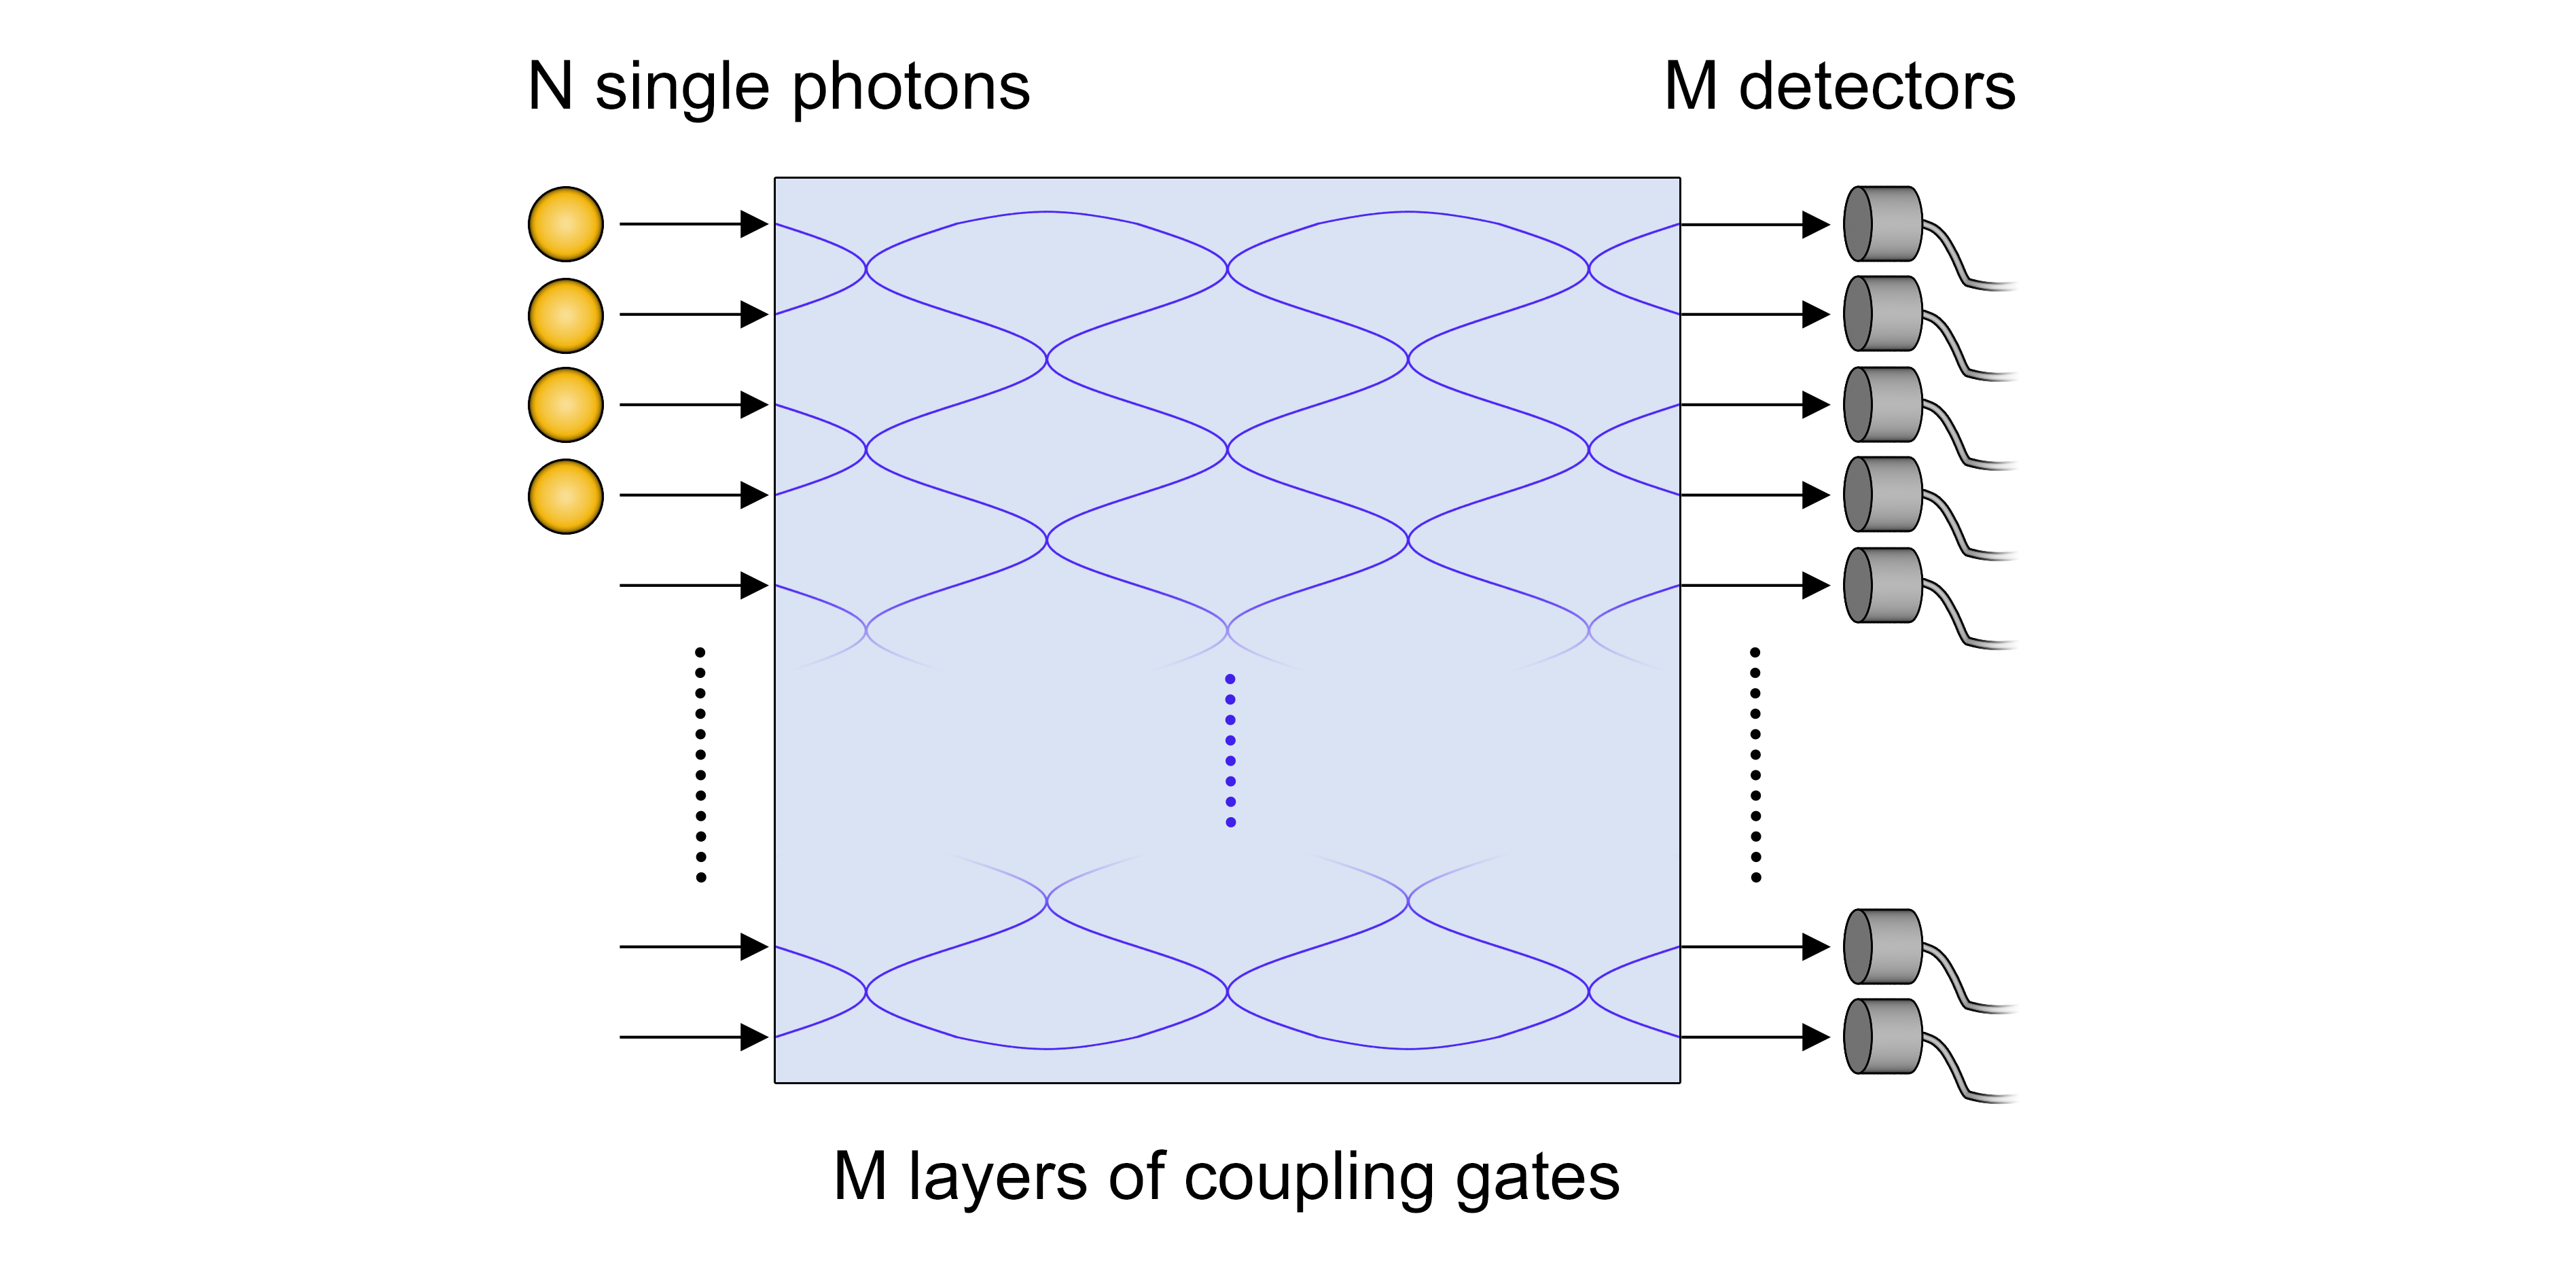
\includegraphics[width=16cm]{figures/1712.10037v3.png}\vspace{-0.2cm}
\caption{In a boson sampling device N single photons are sent over an M mode linear optical circuit composed of M layers of two-mode coupling gates and detected at the output with photon counting detectors. \cite{dede}}
\label{fig:bosonsample}
\end{figure}

\section{Preliminaries}
\subsection{The Fock States and the Fock Space}
Consider a quantum system where we have multiple identical quantum particles, each occupying a state within a Hilbert space. We want to study the entire multi-particle system and its states.

For example, if we have a system that contains two bosonic particles, where each of their states is described by a wave function \( |\psi_1\rangle \) and \( |\psi_2\rangle \) in the Hilbert space, then the entire state of the system (constructed from boson 1 and boson 2 respectively) can be described as the tensor product of these two states:

\begin{equation}
|\psi_{1,2}\rangle = |\psi_1\rangle \otimes |\psi_2\rangle
\end{equation}

However, if the two particles are identical bosons, we cannot distinguish which particle is in which state anymore. This means that for the multi-particle system, there should be an equal probability of finding particle 1 in state \( x_1 \) and particle 2 in state \( x_2 \), and vice versa. Therefore:

\begin{equation}
|\psi_{12}\rangle = |\psi_1\rangle \otimes |\psi_2\rangle
\end{equation}

should be equal to finding particle 2 in state \( x_2 \) and particle 1 in state \( x_1 \):

\begin{equation}
|\psi_{21}\rangle = |\psi_2\rangle \otimes |\psi_1\rangle
\end{equation}

Thus, we have:

\begin{equation}
|\psi_{12}\rangle = |\psi_{21}\rangle
\end{equation}

Introducing this symmetry should be ensured in the multi-particle system:

\begin{equation}
|\psi\rangle = \frac{1}{\sqrt{2}} \left( |\psi_1\rangle \otimes |\psi_2\rangle + |\psi_2\rangle \otimes |\psi_1\rangle \right)
\end{equation}

Here, the Fock space comes into play to introduce the second quantization representation, which focuses on the number of particles in each possible state, rather than which particle occupies which state (as in the first quantization representation).

A \textbf{Fock state} \( |F\rangle \) represents the infinite occupation numbers of particles in \textbf{all possible state of the Hilbert space} \( |u_i\rangle \). The occupation number \( n_i \) corresponds to the number of particles occupying the \( i \)-th quantum state \( |u_i\rangle \).

For example, if the state \( |u_1\rangle \) is occupied by \( n_1 \) particles, the Fock state can be written as:

\begin{equation}
|F\rangle = |n_1, n_2, \dots, n_i, \dots \rangle
\end{equation}

where \( n_1, n_2, \dots \) are the occupation numbers for the respective quantum states \( |u_1\rangle, |u_2\rangle, \dots \). In the case of bosons, the occupation numbers \( n_i \) can take any non-negative integer value, representing the number of bosons occupying each state.



\subsection{The Permanent of a Matrix}

The permanent is a function applied only to square matrices. It is calculated similarly to the determinant but without taking into consideration the sign of the matrix elements (all terms are considered positive). The formula for the permanent of an \( n \times n \) matrix \( A = [a_{ij}] \) is:

\begin{equation}
\text{perm}(A) = \sum_{\sigma \in S_n} \prod_{i=1}^{n} a_{i,\sigma(i)}
\end{equation}

where \( S_n \) is the set of all permutations of \( \{1, 2, \dots, n\} \), and \( \sigma \) represents a permutation.

\subsection{The Haar Unitary Matrix}

A Haar unitary matrix is a random unitary matrix generated from the Haar measure, which is defined as the only uniformly distributed group of unitary matrices. Generating a Haar unitary matrix means producing a random matrix that remains unitary.


\section{The Uncertainty of the Boson Sampling Quantum System}

Shi et al. in \cite{shi_Twa3na} designed a Quantum Random Number Generator (QRNG) based on boson sampling, exploiting its inherent randomness to output true random numbers.

In this system, \( N \)-photons represented by Fock states are introduced into a randomly configured optical network of beam splitters and interferometers, modeled by a Haar unitary matrix \( U \). The output state (also expressed in Fock states) \( \ket{\psi_{\text{out}}} \) represents the probability of detecting \( j_i \) photons by the \( i \)-th detector. This probability can be calculated using the following formula:


\begin{equation}
    P(\mathbf{j}) = \frac{\left| \operatorname{Perm}(U_{\mathbf{j}}) \right|^2}{\prod_{i=1}^{m} j_i!}
\end{equation}





where \( \operatorname{Perm}(U_{\mathbf{j}}) \) is the permanent of the submatrix \( U_{\mathbf{j}} \) corresponding to the input and output modes, and \( \mathbf{j} = (j_1, j_2, \dots, j_m) \) is the output configuration with \( j_i \) photons detected at the \( i \)-th mode.

Shi et al. used single-photon detectors, which are easier to implement physically. Each detector collects whether there is a photon at that mode (or multiple photons) or not, providing the bitstring representation needed for random number generation.

The output of this boson sampling system is a superposition of all possible Fock states:


\begin{equation}
    \ket{\psi_{\text{out}}} = \sum_i \lambda_i \ket{\psi_i}

\end{equation}    



According to the fundamental randomness of quantum mechanics, when the final state is measured using the detectors, the system collapses randomly to one of the possible states with a probability proportional to the square of the corresponding coefficient \( |\lambda_i|^2 \). Since the bosonic state evolves through beam splitters and interferometers, this randomness increases, making the boson sampling output more suitable as an entropy source for a true random number generator.


\section{The Unreproducibility of the Boson Sampling Quantum System}

The results of the boson sampler are completely independent of the initial input state. The initial input configuration does not affect the output, as the system evolves through a Haar unitary matrix \( U \), representing the randomness introduced by beam splitters and interferometers.

As stated by Shi et al. in \cite{shi_Twa3na}, boson sampling QRNGs cannot be efficiently simulated as the output size increases. This is due to the computational complexity of calculating the \textbf{permanent of a matrix}, which grows exponentially with the system size. The permanent calculation is essential in describing the system's evolution, making classical simulation infeasible for large-scale boson sampling systems.





\chapter{CQTPost Processor (CQTPP)}
\label{ch3}
The CQT Post Processor (CQTPP) was first introduced by the CQTech team during the ORCA Hackathon. It addresses both bias and autocorrelation reduction in randomly generated numbers that may be biased and correlated (or dependent), unlike the Von Neumann method, which requires the input to be uniformly biased and independent.

The CQTPP algorithm (detailed in the appendices) follows these steps:

\begin{enumerate}
    \item \textbf{Divide the input bitstream} into two equal samples: Sample 1 and Sample 2.
    \item \textbf{Divide each sample into chunks} of a pre-defined size, referred to as the \texttt{dep\_seq\_len} (a hyperparameter).
    \item \textbf{Process the chunks as follows:}
    \begin{itemize}
        \item Take the first chunk from Sample 1 and the first chunk from Sample 2.
        \item For each pair of chunks, take the corresponding bits from both chunks and apply the \textbf{Von Neumann mapping}.
        \item Continue this process until all bits in the chunks are processed (the size of each chunk is \texttt{dep\_seq\_len}).
    \end{itemize}
    \item \textbf{For each pair of chunks}, obtain the Von Neumann processed output.
    \item \textbf{Take only the first bit} of that output and append it to the final result of CQTPP, discarding the remaining bits.
    \item \textbf{Repeat this operation} for all remaining chunks.
\end{enumerate}

This process is illustrated in \textbf{Fig. \ref{fig:CQTPP_process}}.

\begin{figure}[h]
\centering
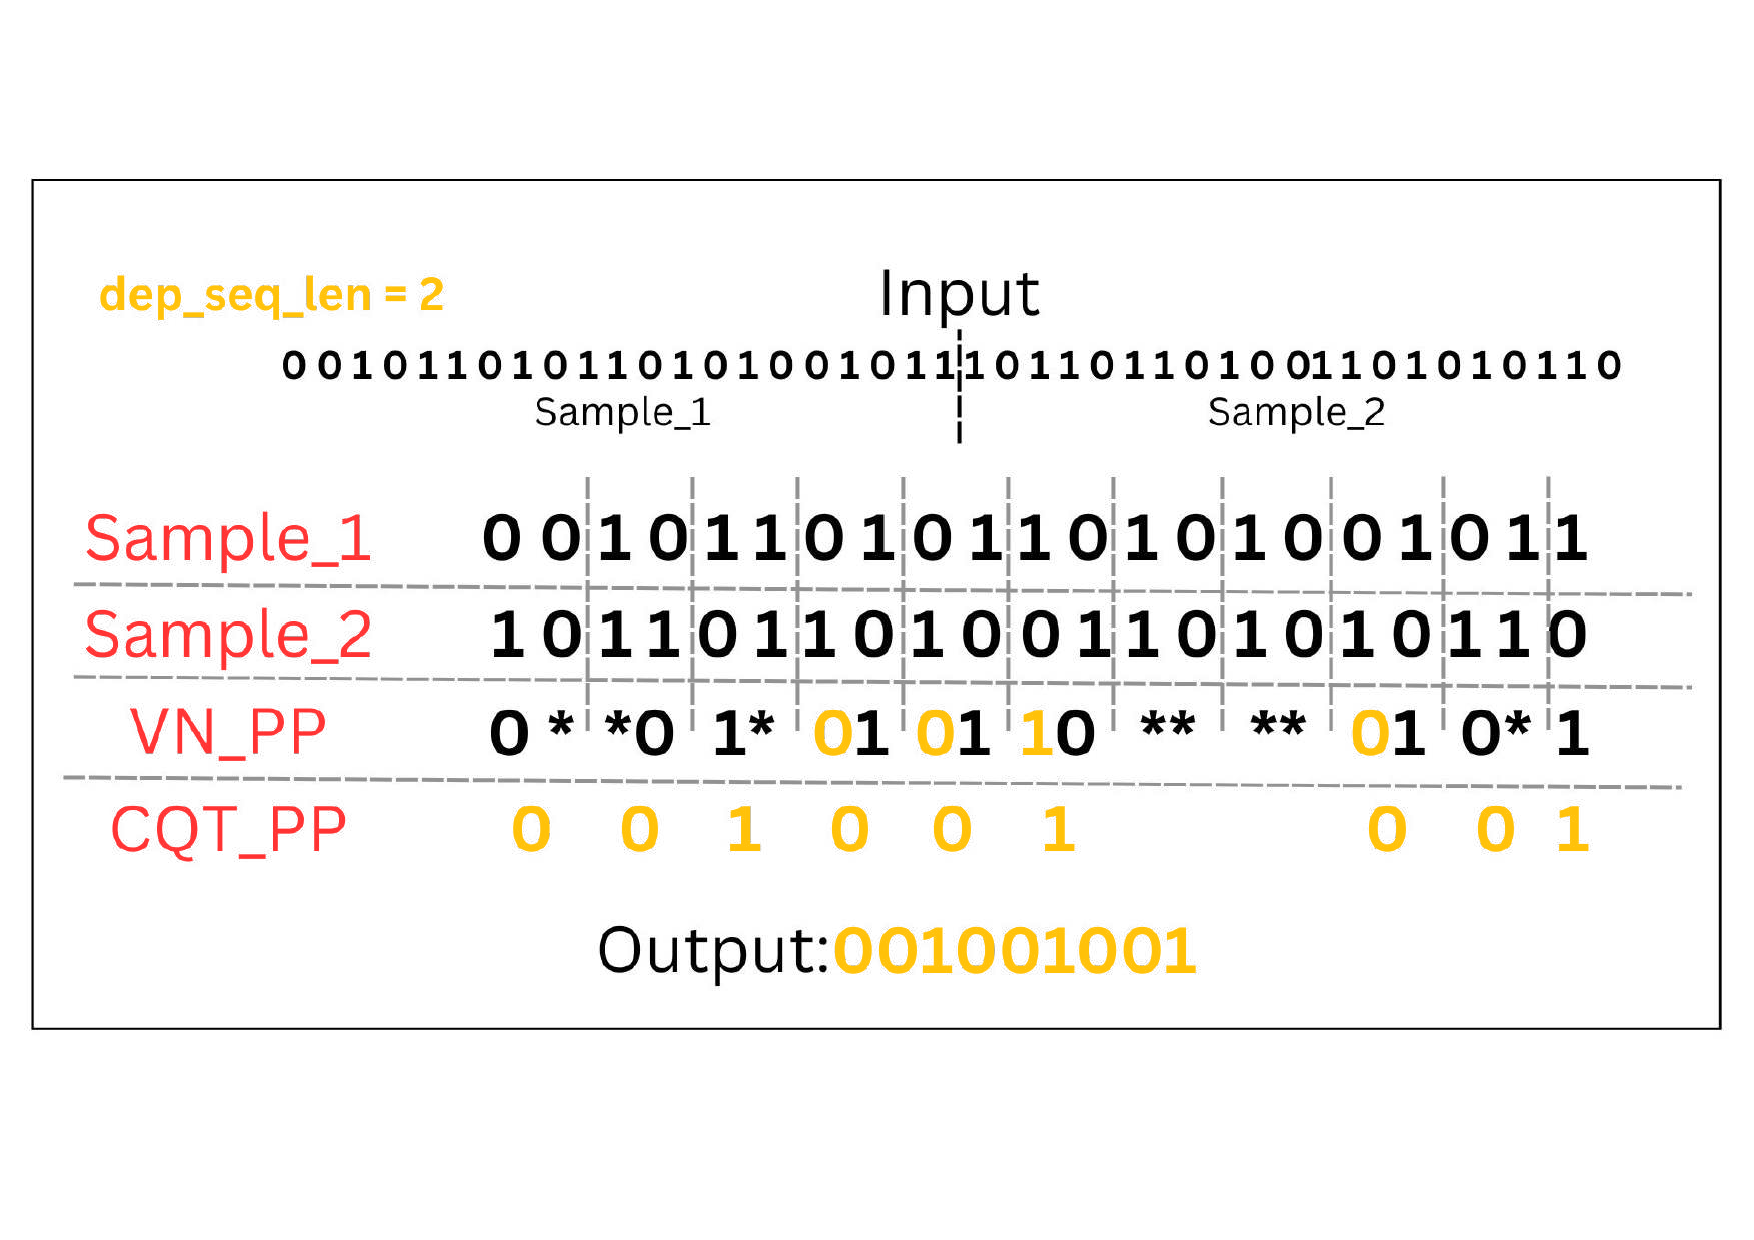
\includegraphics[width=12cm]{figures/CQTPP.pdf}
\caption{Diagram illustrating the process of the CQT Post Processor (CQTPP)}
\label{fig:CQTPP_process}
\end{figure}

\section{Performance and Output Results}

Considering we have a bitstream of length 4, all possible combinations are \(2^4 = 16\). Table~\ref{tab:output_comparison} shows the outputs generated using both the CQT Post Processor (CQTPP) and the Von Neumann Post Processor (VonNeuPP).

\begin{table}[h]
\centering
\caption{Output Comparison Between CQTPP and VonNeuPP}
\label{tab:output_comparison}
\begin{tabular}{|c|c|c|}
\hline
\textbf{Bits} & \textbf{CQTPP Output} & \textbf{VonNeuPP Output} \\ \hline
0000 & X  & X  \\ \hline
0001 & 0  & 0  \\ \hline
0010 & 0  & 0  \\ \hline
0011 & 0  & 00 \\ \hline
0100 & 1  & 1  \\ \hline
0101 & X  & X  \\ \hline
0110 & 0  & 01 \\ \hline
0111 & 0  & 0  \\ \hline
1000 & 1  & 1  \\ \hline
1001 & 1  & 10 \\ \hline
1010 & X  & X  \\ \hline
1011 & 0  & 0  \\ \hline
1100 & 1  & 11 \\ \hline
1101 & 1  & 1  \\ \hline
1110 & 1  & 1  \\ \hline
1111 & X  & X  \\ \hline
\end{tabular}
\end{table}

In the table, \(X\) indicates no output.

As mentioned in previous sections, for a number to be truly random, the probabilities of obtaining a 0 or 1 should be equal. Additionally, the probabilities of obtaining the bit pairs \(00\), \(01\), \(10\), and \(11\) should also be equal.

Let \(p_{00}\), \(p_{01}\), \(p_{10}\), and \(p_{11}\) denote the probabilities that the input bitstream contains the respective pairs \(00\), \(01\), \(10\), and \(11\). For example, the probability that the input bitstream is \(0110\) is given by:
\[
p(\text{0110}) = p_{01} \times p_{10}
\]

To prove the unbiasedness of the output, we need to show that:
\[
p(\text{out} = 0) = p(\text{out} = 1)
\]
and also:
\[
p(\text{out} = 00) = p(\text{out} = 01) = p(\text{out} = 10) = p(\text{out} = 11)
\]

\noindent As proven in the appendix, for the Von Neumann Post Processor:
\[
p(\text{out} = 0) = p(\text{out} = 1)
\]

However, regarding the equal probabilities of bit pairs, we can extract from Table~\ref{tab:output_comparison} the following relationships:

\[
p(\text{out} = 00) = p_{00} \times p_{11}, \quad p(\text{out} = 11) = p_{11} \times p_{00}
\]
\[
p(\text{out} = 01) = p_{01} \times p_{10}, \quad p(\text{out} = 10) = p_{10} \times p_{01}
\]

\noindent Therefore, for the condition to be true, we need to satisfy:
\[
p_{00} \times p_{11} = p_{01} \times p_{10}
\]

\noindent This condition remains true for uncorrelated input data.

\noindent On the other hand, the CQTPP ensures equal probabilities for all possible outputs.

Since the outcomes of CQTPP are only one bit in length, the output matches the Von Neumann Post Processor for 8 cases (excluding the empty output). As previously proven, these cases are equally distributed, and we refer to this probability as \(a\).

For the CQTPP to be unbiased, the following condition must hold:
\[
P(\text{out} = 0) = P(\text{out} = 1)
\]

We can express \(P(\text{out} = 0)\) as:
\[
P(\text{out} = 0) = a + p_{00} \times p_{11} + p_{01} \times p_{10}
\]

Similarly, for \(P(\text{out} = 1)\):
\[
P(\text{out} = 1) = a + p_{11} \times p_{00} + p_{10} \times p_{01}
\]

Therefore, we have:
\[
P(\text{out} = 0) = P(\text{out} = 1)
\]

This equality holds regardless of whether the input data is correlated or independent.

\noindent The same scheme can be extended to larger-scale inputs, with the unbiasedness being preserved.

\section{CQTPP Variants}
In this study, we propose several variants that utilize the same core principles of the CQTPP and aim to improve its results.

\subsection{Iterative CQTPP (ItCQTPP)}
The Iterative CQTPP (ItCQTPP) variant focuses on improving the throughput of the CQTPP by minimizing discarded bits.  
In this scheme, the discarded bits from the Von Neumann output (the remaining bits after applying the CQTPP) are gathered and re-processed through the CQTPP.  
This iterative process allows for a reduction in wasted information, thus slightly increasing the overall efficiency and throughput of the post-processing.  

An illustration of the Iterative CQTPP method is shown in Fig.~\ref{fig:itcqtpp}.

\begin{figure}[h!]
    \centering
    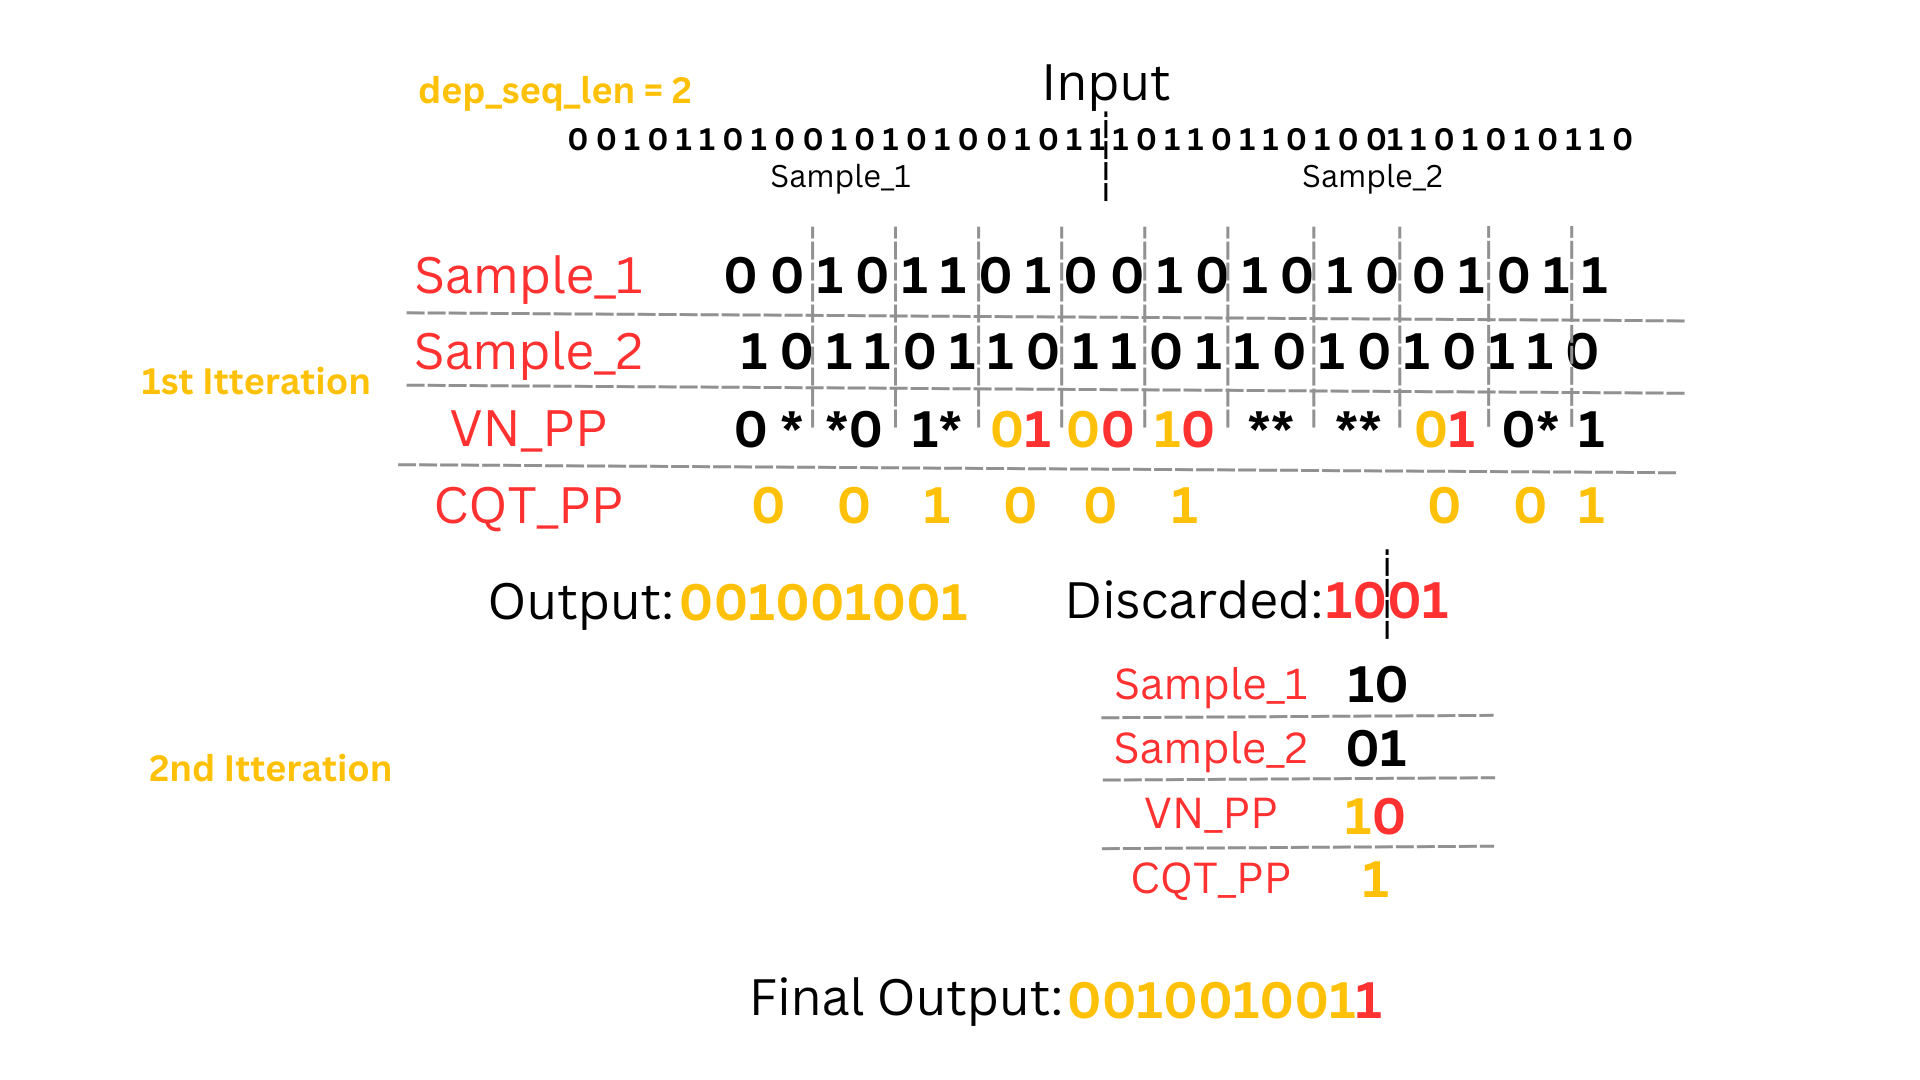
\includegraphics[width=0.8\textwidth]{figures/itcqtpp.png}
    \caption{Illustration of the process of the Iterative CQTPP method (ItCQTPP).}
    \label{fig:itcqtpp}
\end{figure}

\subsection{CQTPP/MKV}
The CQTPP/MKV variant aims to improve the de-correlation performance of the CQTPP by introducing a Markov Chain post-processing step.  
In this scheme, the output of the CQTPP is routed through a Markov Chain with either a 1-bit or 2-bit history.  
This additional step enhances the reduction of autocorrelation in the bitstream, leading to a more uniform and less predictable output.  

The schematic representation of the CQTPP/MKV method is shown in Fig.~\ref{fig:cqtppmkv}.



\begin{figure}[h!]
    \centering
    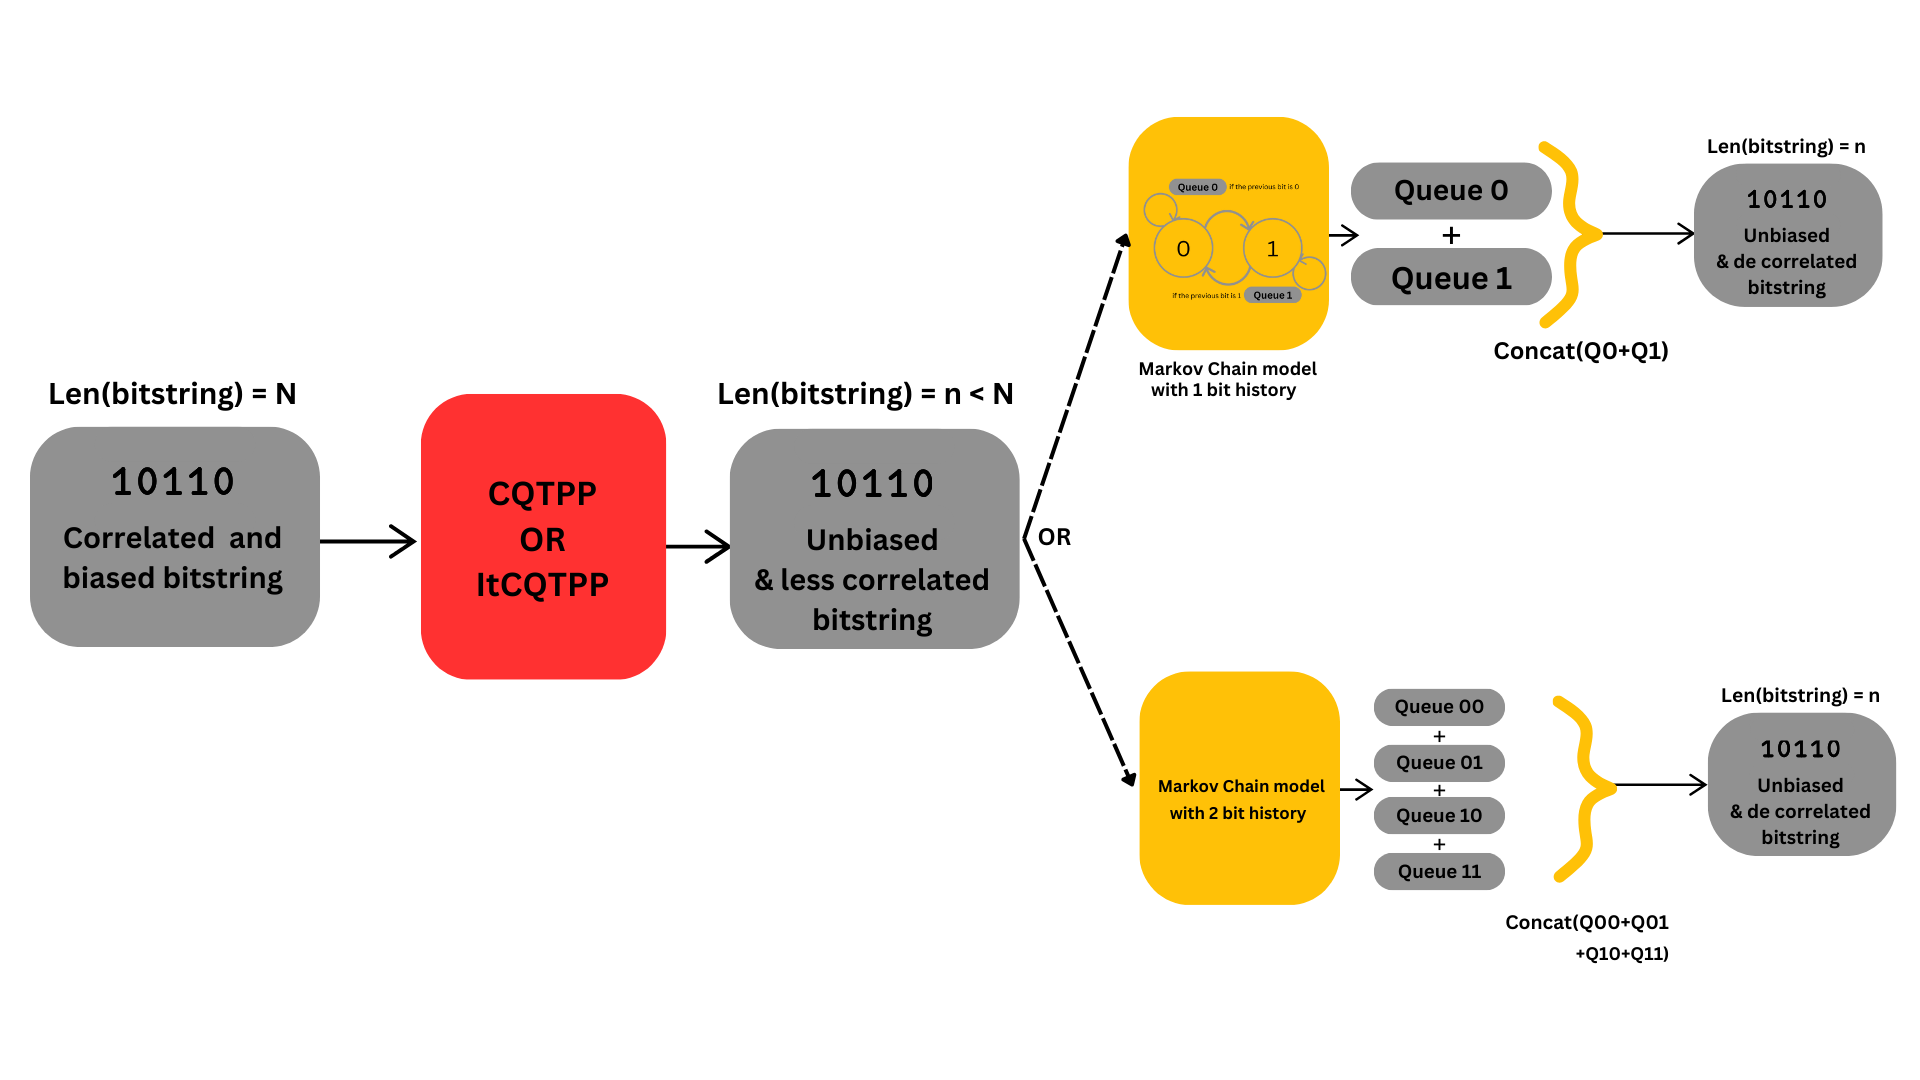
\includegraphics[width=0.8\textwidth]{figures/cqtppmkv.png}
    \caption{Schematic representation of the CQTPP/MKV method.}
    \label{fig:cqtppmkv}
\end{figure}



Now we are going to evaluate the results of the CQTPP and its variant based on the evaluation metrics we set above, and compare them with the Von Neumann Post Processors for different entropy sources sampling and using different hyper-parameters:

\subsection{The Entropy and n-bits Distribution}
Using a Markov model, we generated 20 bitstreams, each of length 10,000 (best for locally used computational power), by setting \( p_0 \), the probability that each bit is 0, and the autocorrelation coefficient \( \phi_1 \), which changes the nature of the entropy source as we can see in Table \ref{tab:experiments}.

\begin{table}[h!]
    \centering
    \begin{tabular}{|c|c|c|l|}
        \hline
        \textbf{Experiment} & \textbf{\( p_0 \)} & \textbf{Correlation Coefficient (\( \phi_1 \))} & \textbf{Remarks on the Nature} \\
        \hline
        A & 0.5 & 0 & Unbiased and independent \\
        B & 0.7 & 0 & Biased but independent \\
        C & 0.6 & 0.4 & Biased and autocorrelated \\
        D & 0.7 & 0.5 & Another biased and autocorrelated  \\
        \hline
    \end{tabular}
    \caption{Entropy source configurations for different experiments.}
    \label{tab:experiments}
\end{table}

The results are shown in Fig. \ref{fig:grph1}.

\begin{figure}[h!]
    \centering
    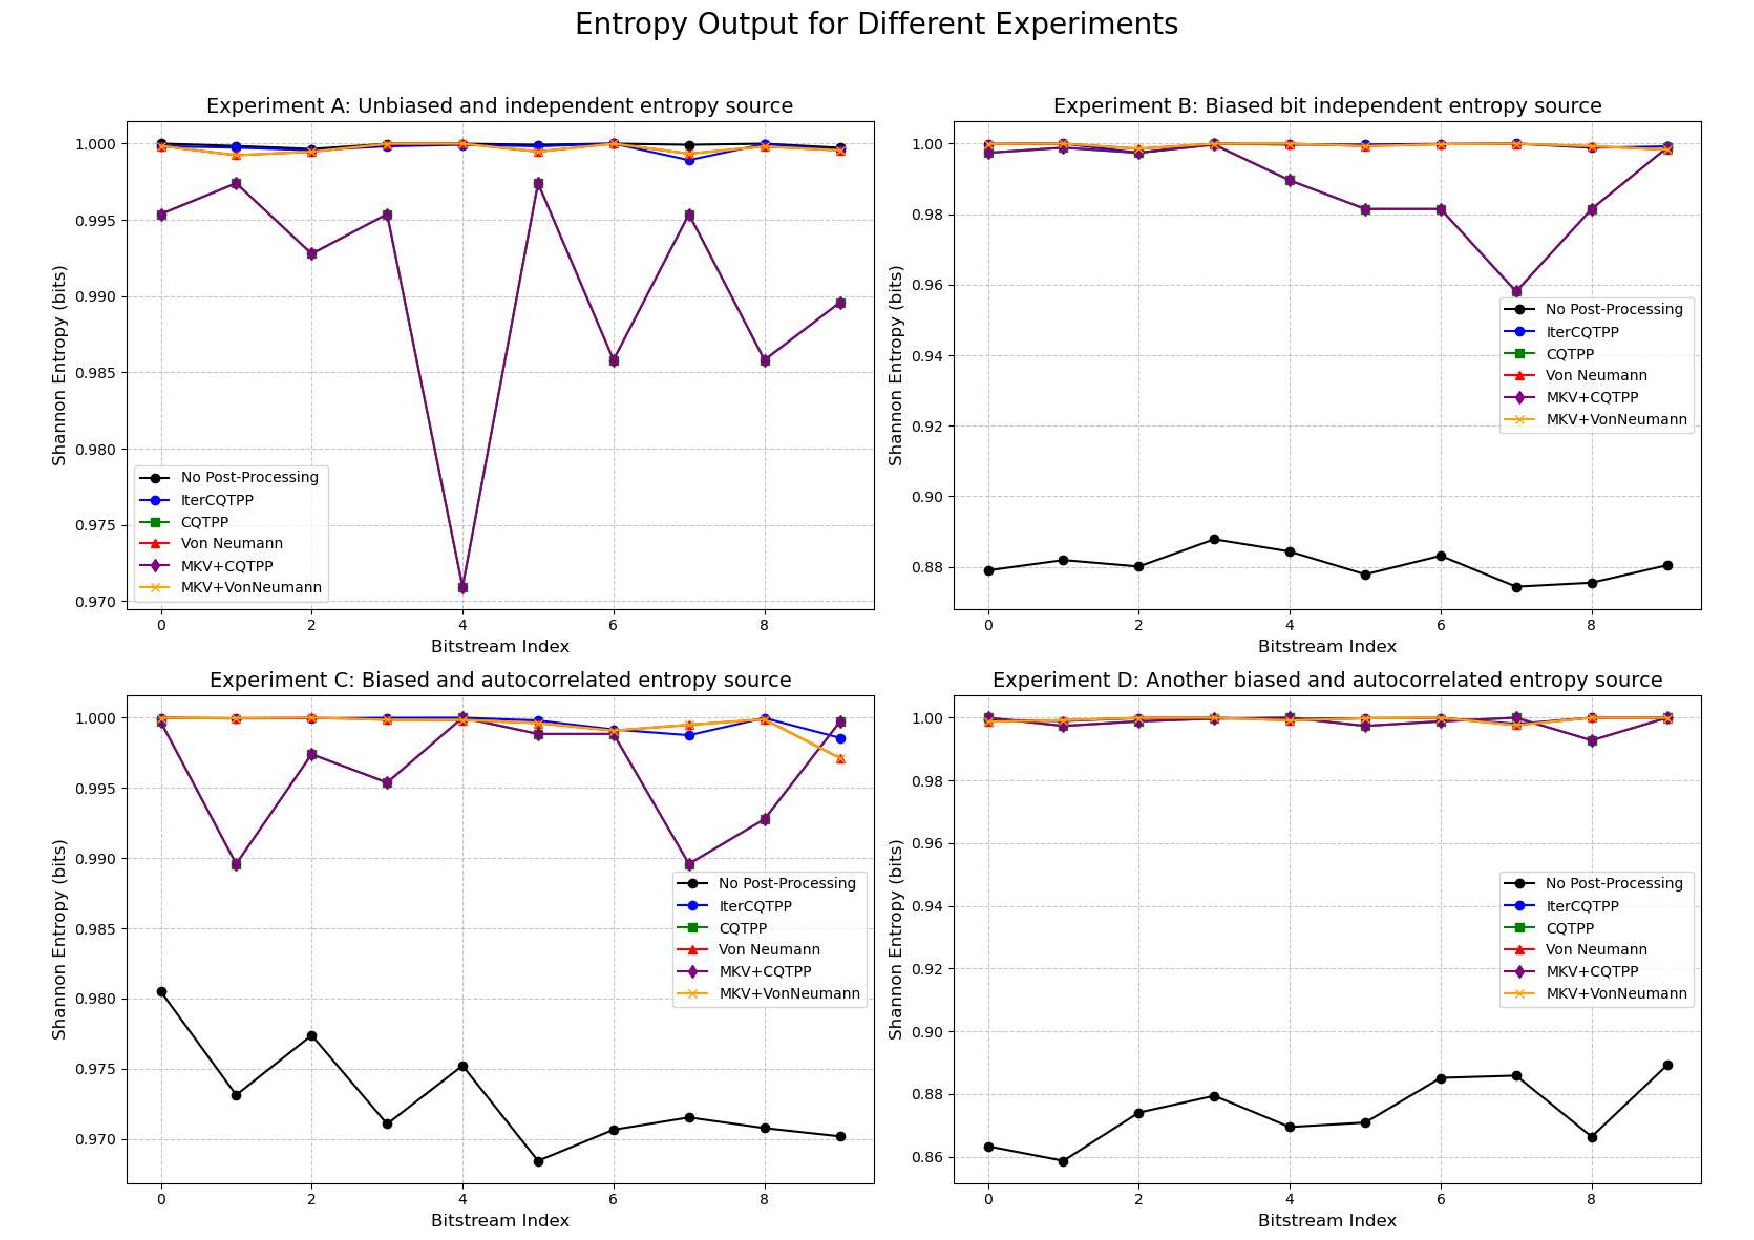
\includegraphics[width=\textwidth]{figures/download.pdf}
    \caption{Entropy output for different experiments using different post processors.}
    \label{fig:grph1}
\end{figure}

We can see that all the post processors and their variants performed well in increasing the entropy. The MKV+CQTPP shows some variance in results in the unbiased and independent bitstream, but it performed well in the other experiments when the autocorrelation increased.

Results distributions are shown in Fig. \ref{fig:grph2}.
Note: Reults will tend to be more unifrom whhen the bit length increases (we couldn't achieve that for computaional reasons)

\begin{figure}[h!]
    \centering
    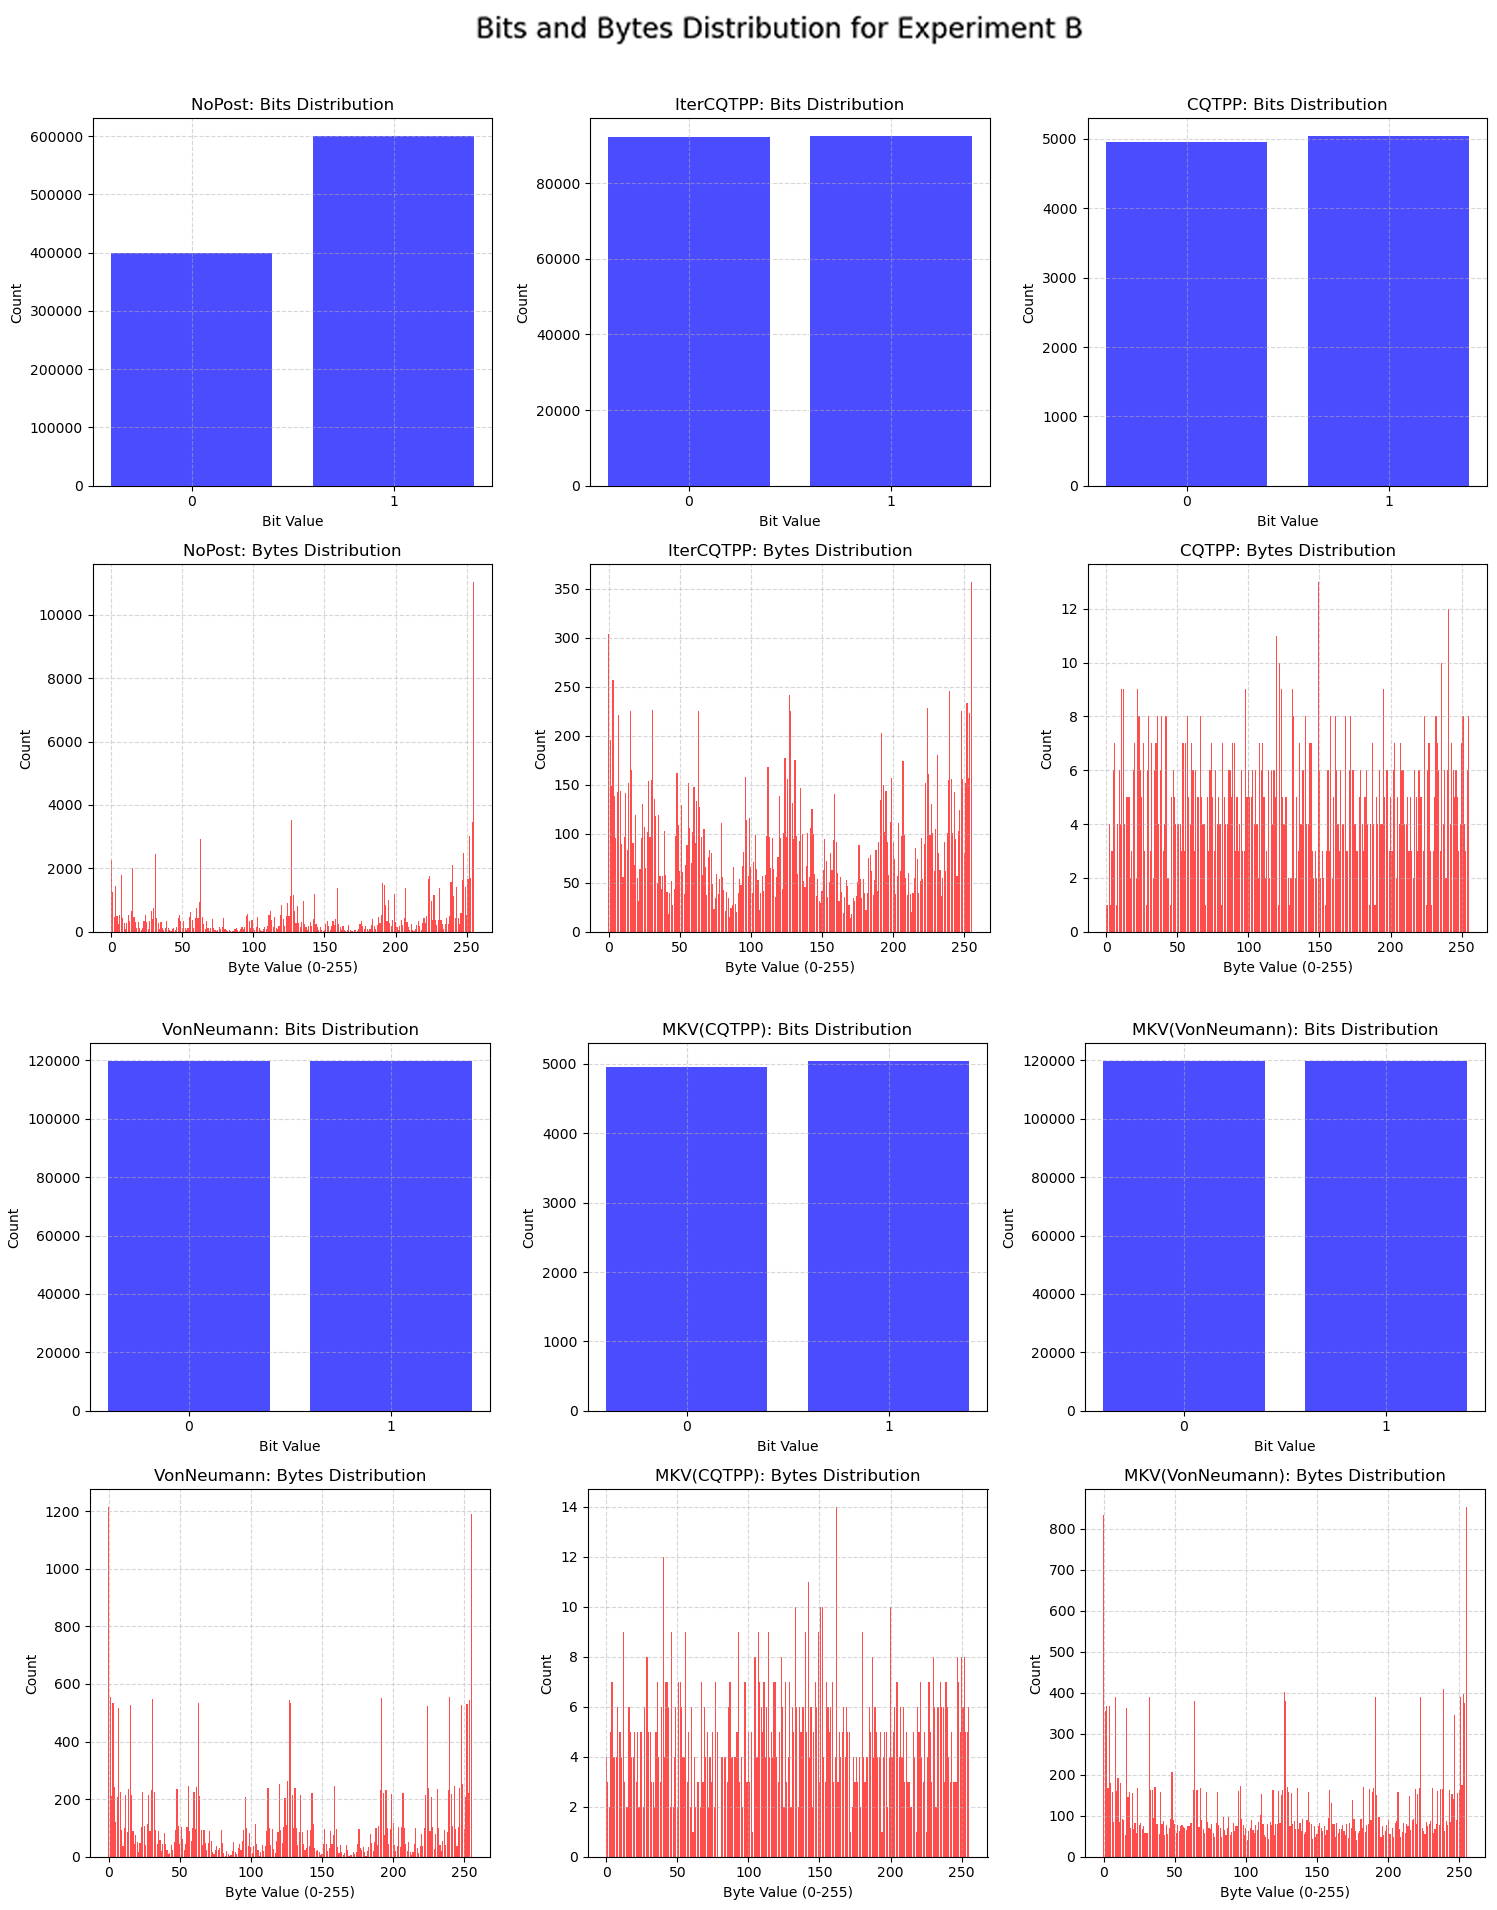
\includegraphics[width=\textwidth]{figures/ExperimentB Dists.png}
    \caption{Bits and Bytes Distribution Experiment C}
    \label{fig:grph2}
\end{figure}

We explore now the results with Real Borealis Data shared by Xanadu in \cite{data}

\noindent Results distributions are shown in Fig. \ref{fig:grph3}.

\begin{figure}[h!]
    \centering
    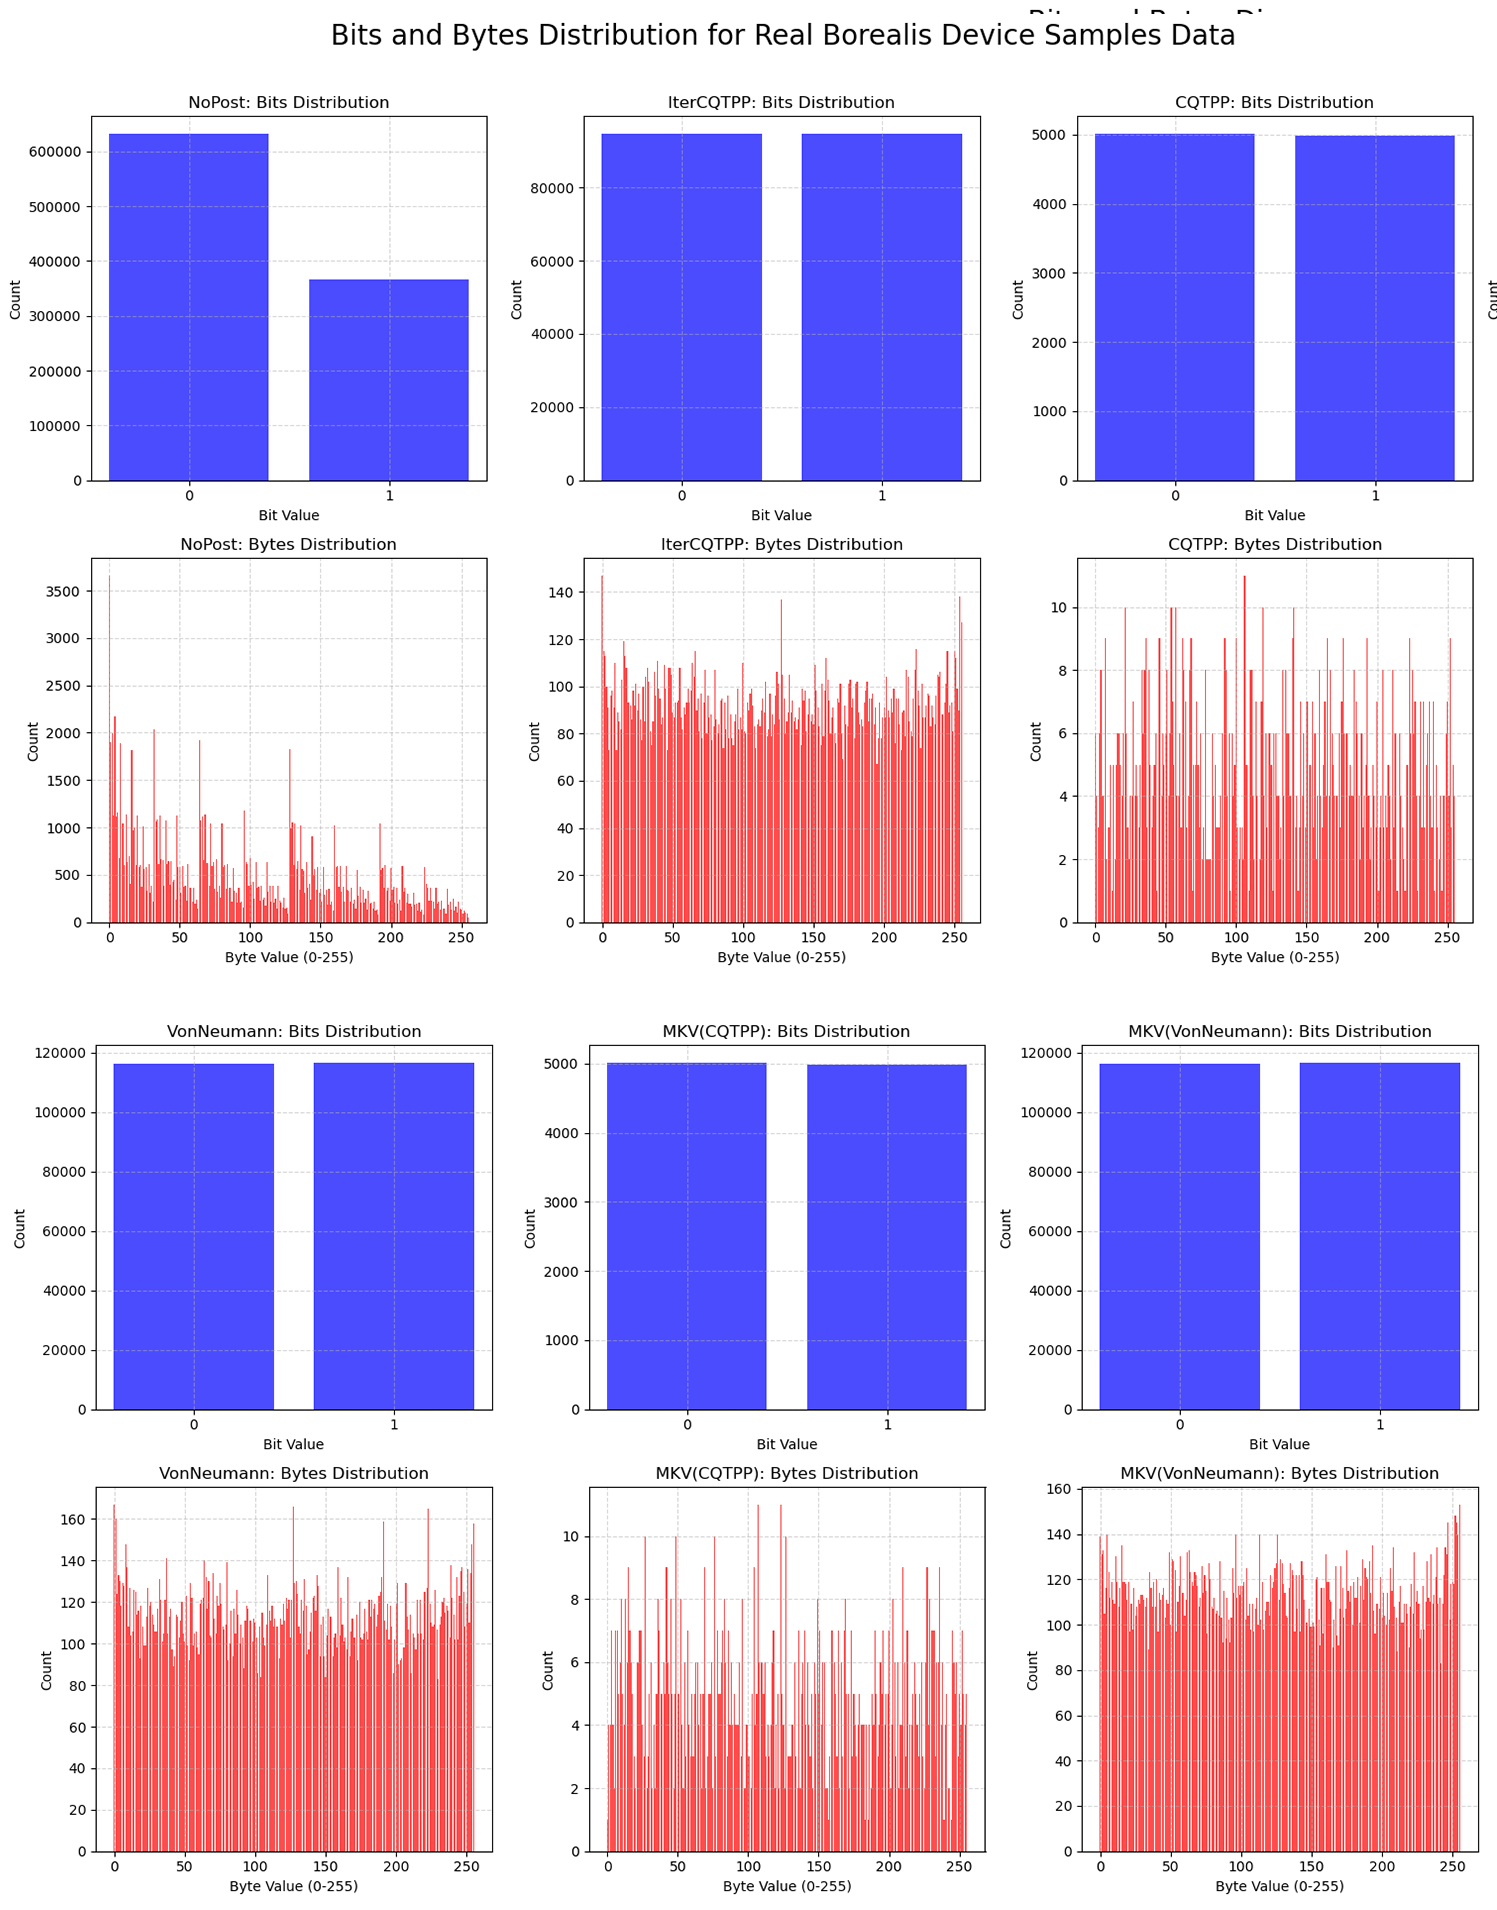
\includegraphics[width=\textwidth]{figures/BorealisResults Dist.png}
    \caption{Bits and Bytes Distribution for Real Borealis Data}
    \label{fig:grph3}
\end{figure}


\subsection{The Autocorrelation:}

Using experiment A2 and B2 explained in the \ref{tab:experiments2} we draw the following results for 20 bitstreams 

\begin{table}[h!]
    \centering
    \begin{tabular}{|c|c|l|}
        \hline
        \textbf{Experiment} & \textbf{\( p_0 \)} & \textbf{Correlation Coefficient (\( \phi_1 \))}  \\
        \hline
        A2 & 0.5 & 0.4 \\
        B2 & 0.5 & 0.7 \\

        \hline
    \end{tabular}
    \caption{Entropy source configurations for different experiments.}
    \label{tab:experiments2}
\end{table}

for lag k = 1 we have results in \ref{fig:grph4}

\begin{figure}[h!]
    \centering
    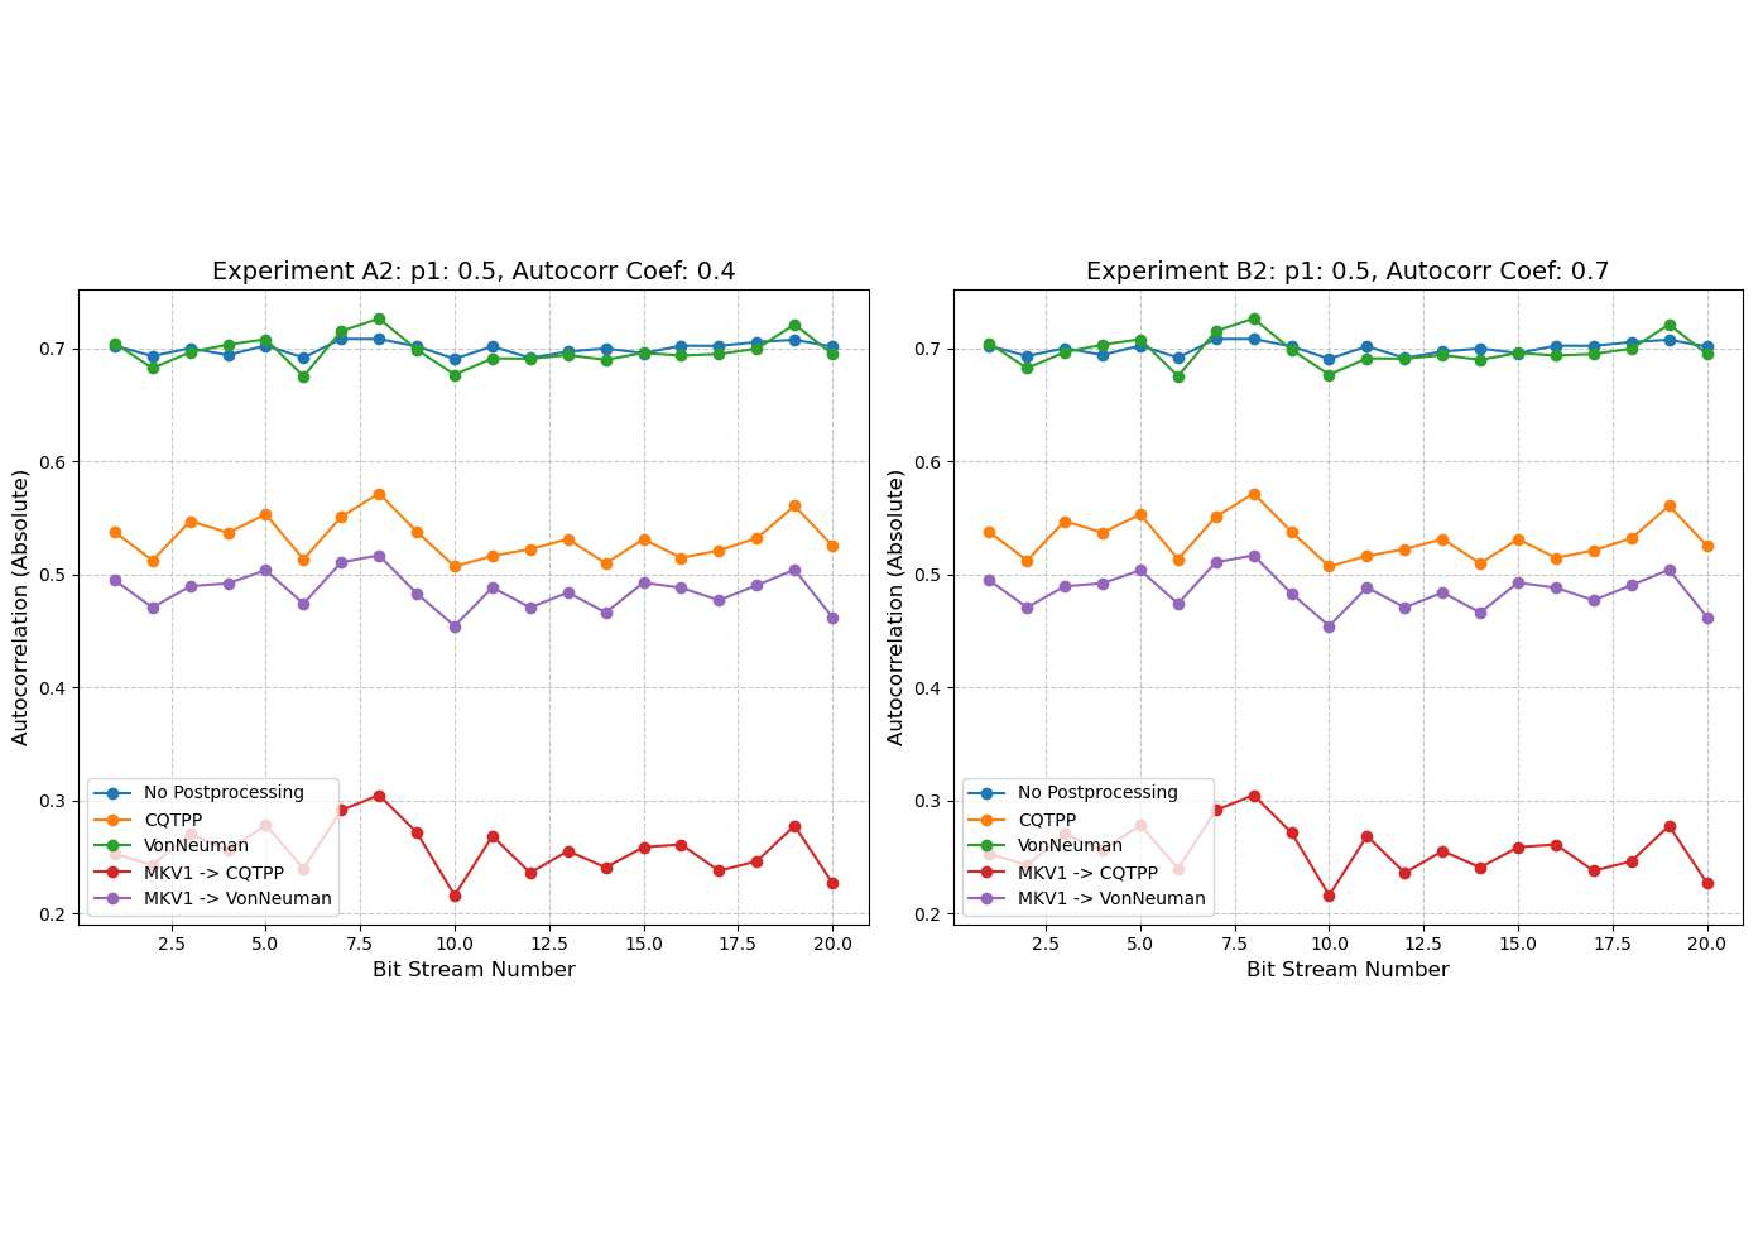
\includegraphics[width=\textwidth]{figures/AutoCorr.pdf}
    \caption{Autocorrealtion with lag k=1 in different bitsrreams using difernet post processors}
    \label{fig:grph4}
\end{figure}

\noindent for lag k = 2 we have results in \ref{fig:grph5}

\begin{figure}[h!]
    \centering
    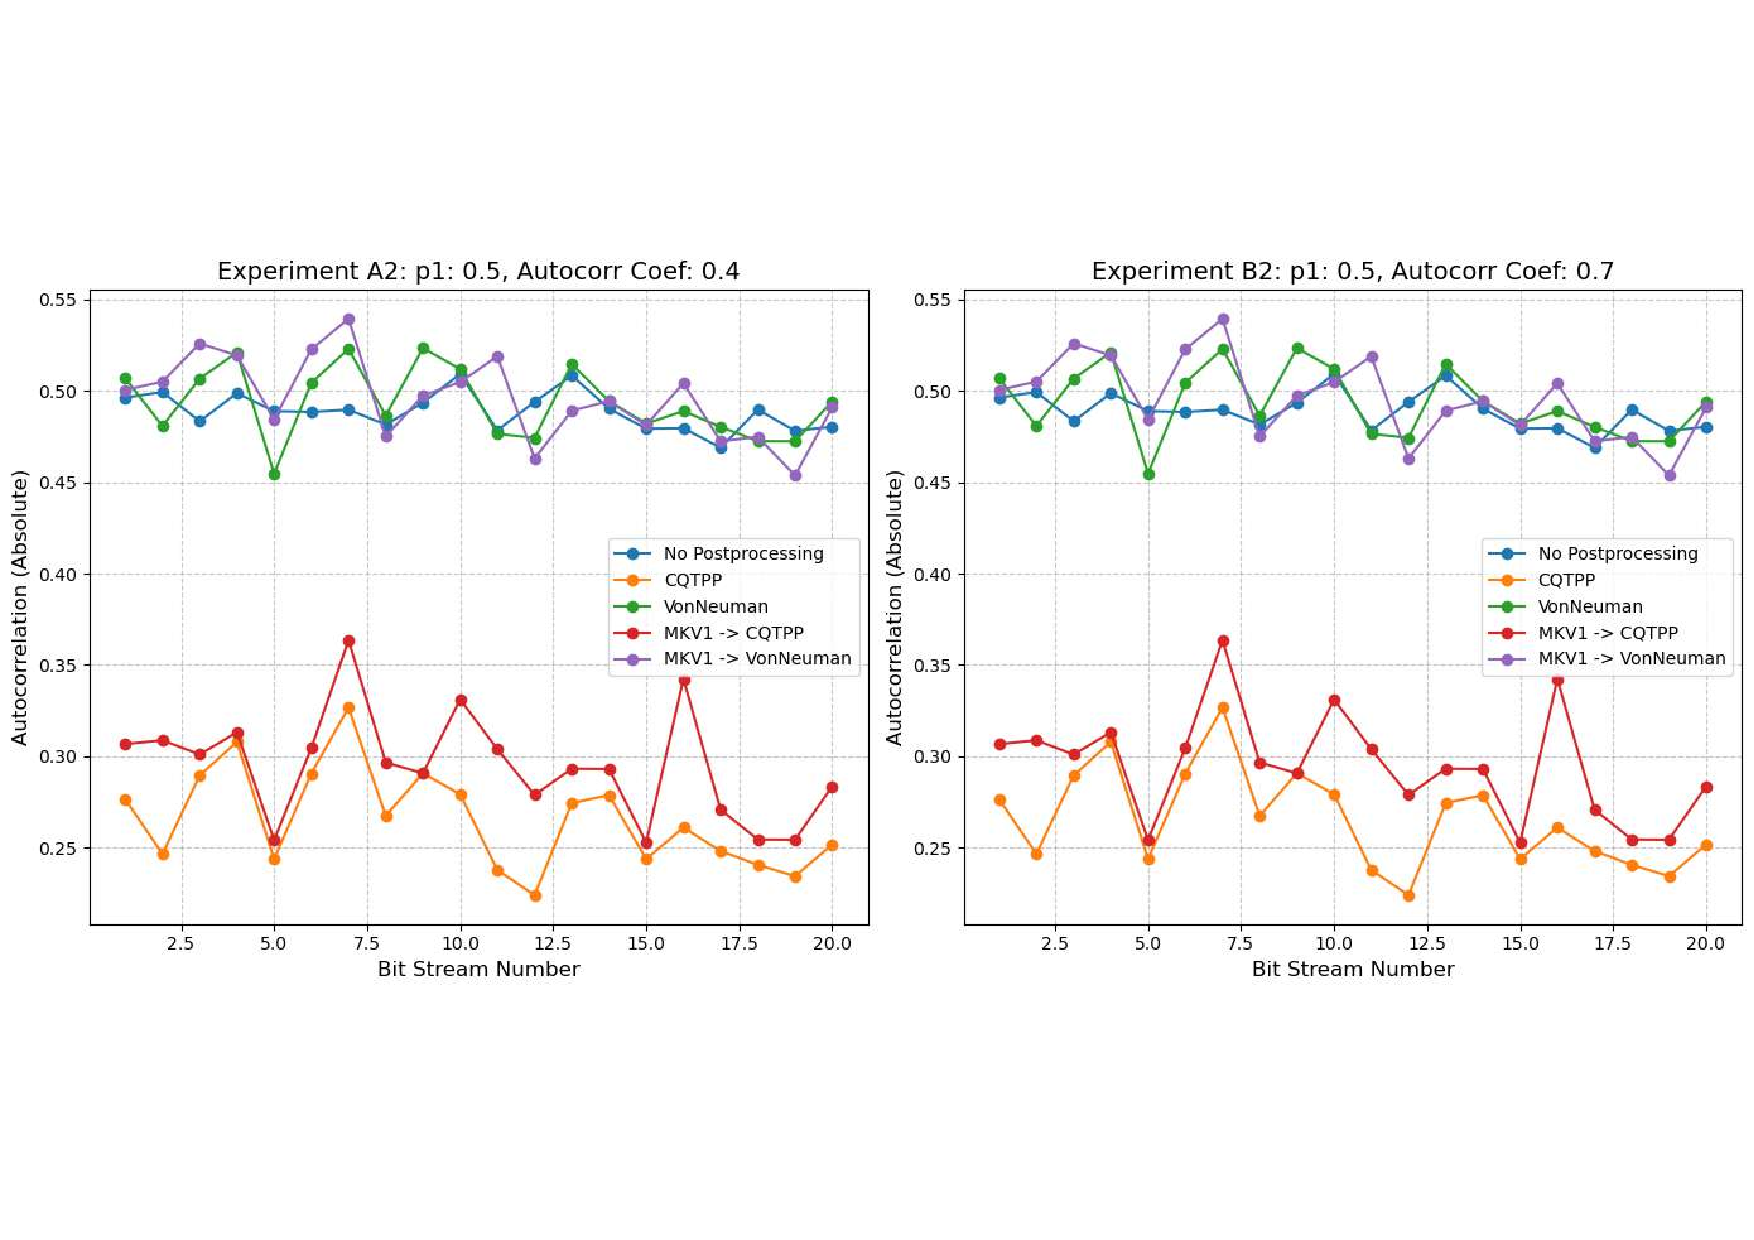
\includegraphics[width=\textwidth]{figures/AutoCorrLag2.pdf}
    \caption{Autocorrealtion with lag k=2 in different bitsrreams using difernet post processors}
    \label{fig:grph5}
\end{figure}

We can see from the results that the CQTPP+MKV achieves excellent results in decorrelating the input bitstream. The CQTPP achieves similar levels of decorrelation as the Von Neumann + MKV model, while the classical Von Neumann Post Processor gives the same autocorrelation results as the input.



\subsection{The Extraction Efficiency}

We calculated the extraction efficiency (ExE) of our post processors for different bitstream lengths. The results are shown in Fig. \ref{fig:grph6}.

\begin{figure}[h!]
    \centering
    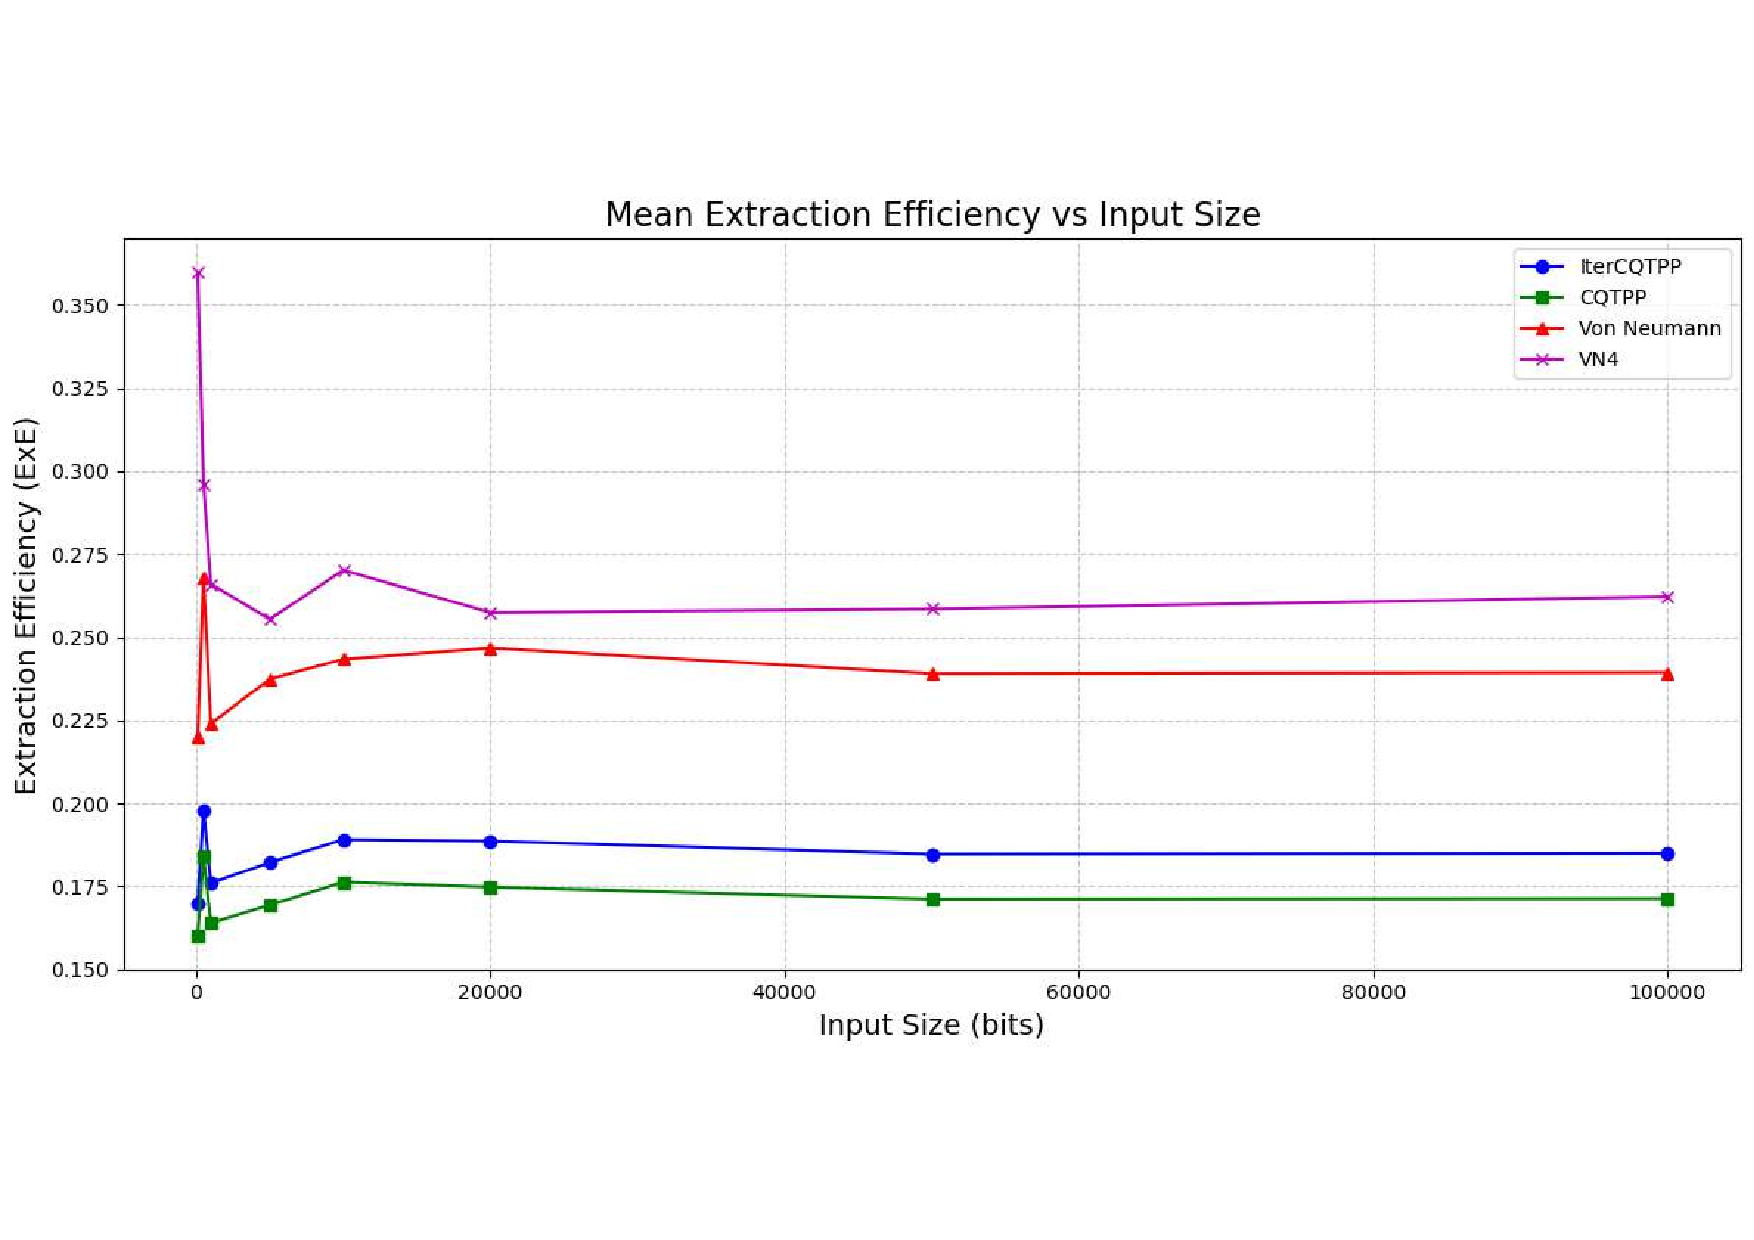
\includegraphics[width=\textwidth]{figures/ExE all.pdf}
    \caption{Extraction Efficiency (ExE) vs. Bitstream Length}
    \label{fig:grph6}
\end{figure}

Each of the post processors' ExE values converges to their theoretical ExE values. As we can see, the Von Neumann Post Processor with 4-bit chunks achieved the highest ExE. Meanwhile, the Iterative CQTPP (IterCQTPP) with 10 iterations provided slightly better results compared to the classical CQTPP.

Note: The combined post processors that include the Markov Chain were not included, since the Markov model does not affect the extraction rate of the bitstream.

\subsection{Remarks and Future Points to Be Exploited}

\textbf{1.} When working on exploring how to improve the throughput of the CQTPP, I noticed that there is a pattern of probabilities produced by the Von Neumann Post-Processor if we only look at the output of the same size. The CQTPP takes only the first bit, and by extracting the general pattern where the sum of the probabilities in sequences starting with the same bit and with the same length are equal (or converge to be so).

We can refine this further where I noticed that we could divide the output of VNPP that have the same length into three clusters, where if we take the sum of a portion of frequencies from each cluster, we can achieve similar probabilities without taking only the first bit. After reading the VN\_N technique \cite{zonga} more thoroughly, I think there might be some similarity between the proposed idea and it — though I’m not entirely sure. This point needs more work and investigation.

\textbf{2.} Another point that can also be exploited is to change the Von Neumann Post-Processor used in the CQTPP to one of its variants (We may use the VN\_8+Waiting strategy since it has a good rate according to \cite{zonga}). These variants will increase the rate of the Von Neumann output and, consequently, the rate of discarded bits produced by it in the CQTPP. Therefore, the Iterative CQTPP will significantly raise its throughput rate.

\chapter{CQT\_RNG Package}
\label{ch4}
\section{The Package}

\texttt{CQT\_RNG} is a library designed to implement and showcase the capability of quantum computers and their underlying quantum principles to generate truly random numbers, aiming to solve the problems of classical random number generators and their reproducibility.


This package is flexible and uses an abstract model to ensure its extendability.


The original codebase for the library can be found on GitHub in \cite{git}

To accompany this study, a new version with improvements and additional modules is presented as \texttt{cqt\_rng\_2.0}, with a class diagram shown in Fig. \ref{fig:UML}.



The package contains the following files and directories:

\begin{itemize}
    \item \textbf{\texttt{base/RNG}}: The main module that gathers The EntropySource with PostProcessor to generate a random bitlist
    \item \textbf{\texttt{base/Evaluator}}: An object to evaluate the randomness of an RNG object in terms of three possible metrices: Extraction Efficency: "ExE", Autocorrelation at lag k:"AutoCorr",Shanon Entropy for n-bit size:"Entropy"
    \item \textbf{\texttt{entropy\_sources/}}: This folder contains different sources used to generate quantum random numbers.
    \begin{itemize}
        \item \textbf{\texttt{real\_devices/}}: Contains modules for generating random data using real quantum devices.
        
        \item \textbf{\texttt{simulators/}}: Contains modules for generating random values using simulations without the need for quantum hardware.
        \begin{itemize}
            \item \texttt{BosonSampler}:Uses the theoretical formulations to genrate data like the Boson Sampler
            \item \texttt{ShiSFSampler}
            \item \texttt{UniversalQCSampler}: Using Pennlyane and universal quantum principles
            \item \texttt{shi_pennylane_sf_sampler}: Pennylane implementation of Shi et al Boson Sampler \cite{shi_Twa3na}
            \item  \texttt{MarkovSampler}: Using the Markov model to generate raw data with certain defined degree of correlation and biasdness
        \end{itemize}
    \end{itemize}
    \item \textbf{\texttt{post\_processors/}}: This folder contains various techniques used for post-processing the generated random data to refine it and achieve a uniform distribution.
    \begin{itemize}
        \item \texttt{VonNeumannPP}
        \item \texttt{CQT\_PP}
        \item \texttt{IterCQT\_PP}: Itterative CQTPP
        \item \texttt{MKV1} using markov model with 1-bit history to remove correlation
        \item \texttt{MKV2} using markov model with 1-bit history to remove correlation
        \item \texttt{CombinedPP}: Uses two PostProcceros and apply them successively on the input bitstring
        \item \texttt{NoPostProcessor}: Yes exactly... that's it :0
    \end{itemize}
\end{itemize}


\begin{landscape}
    \begin{figure}[h!]
    \centering
    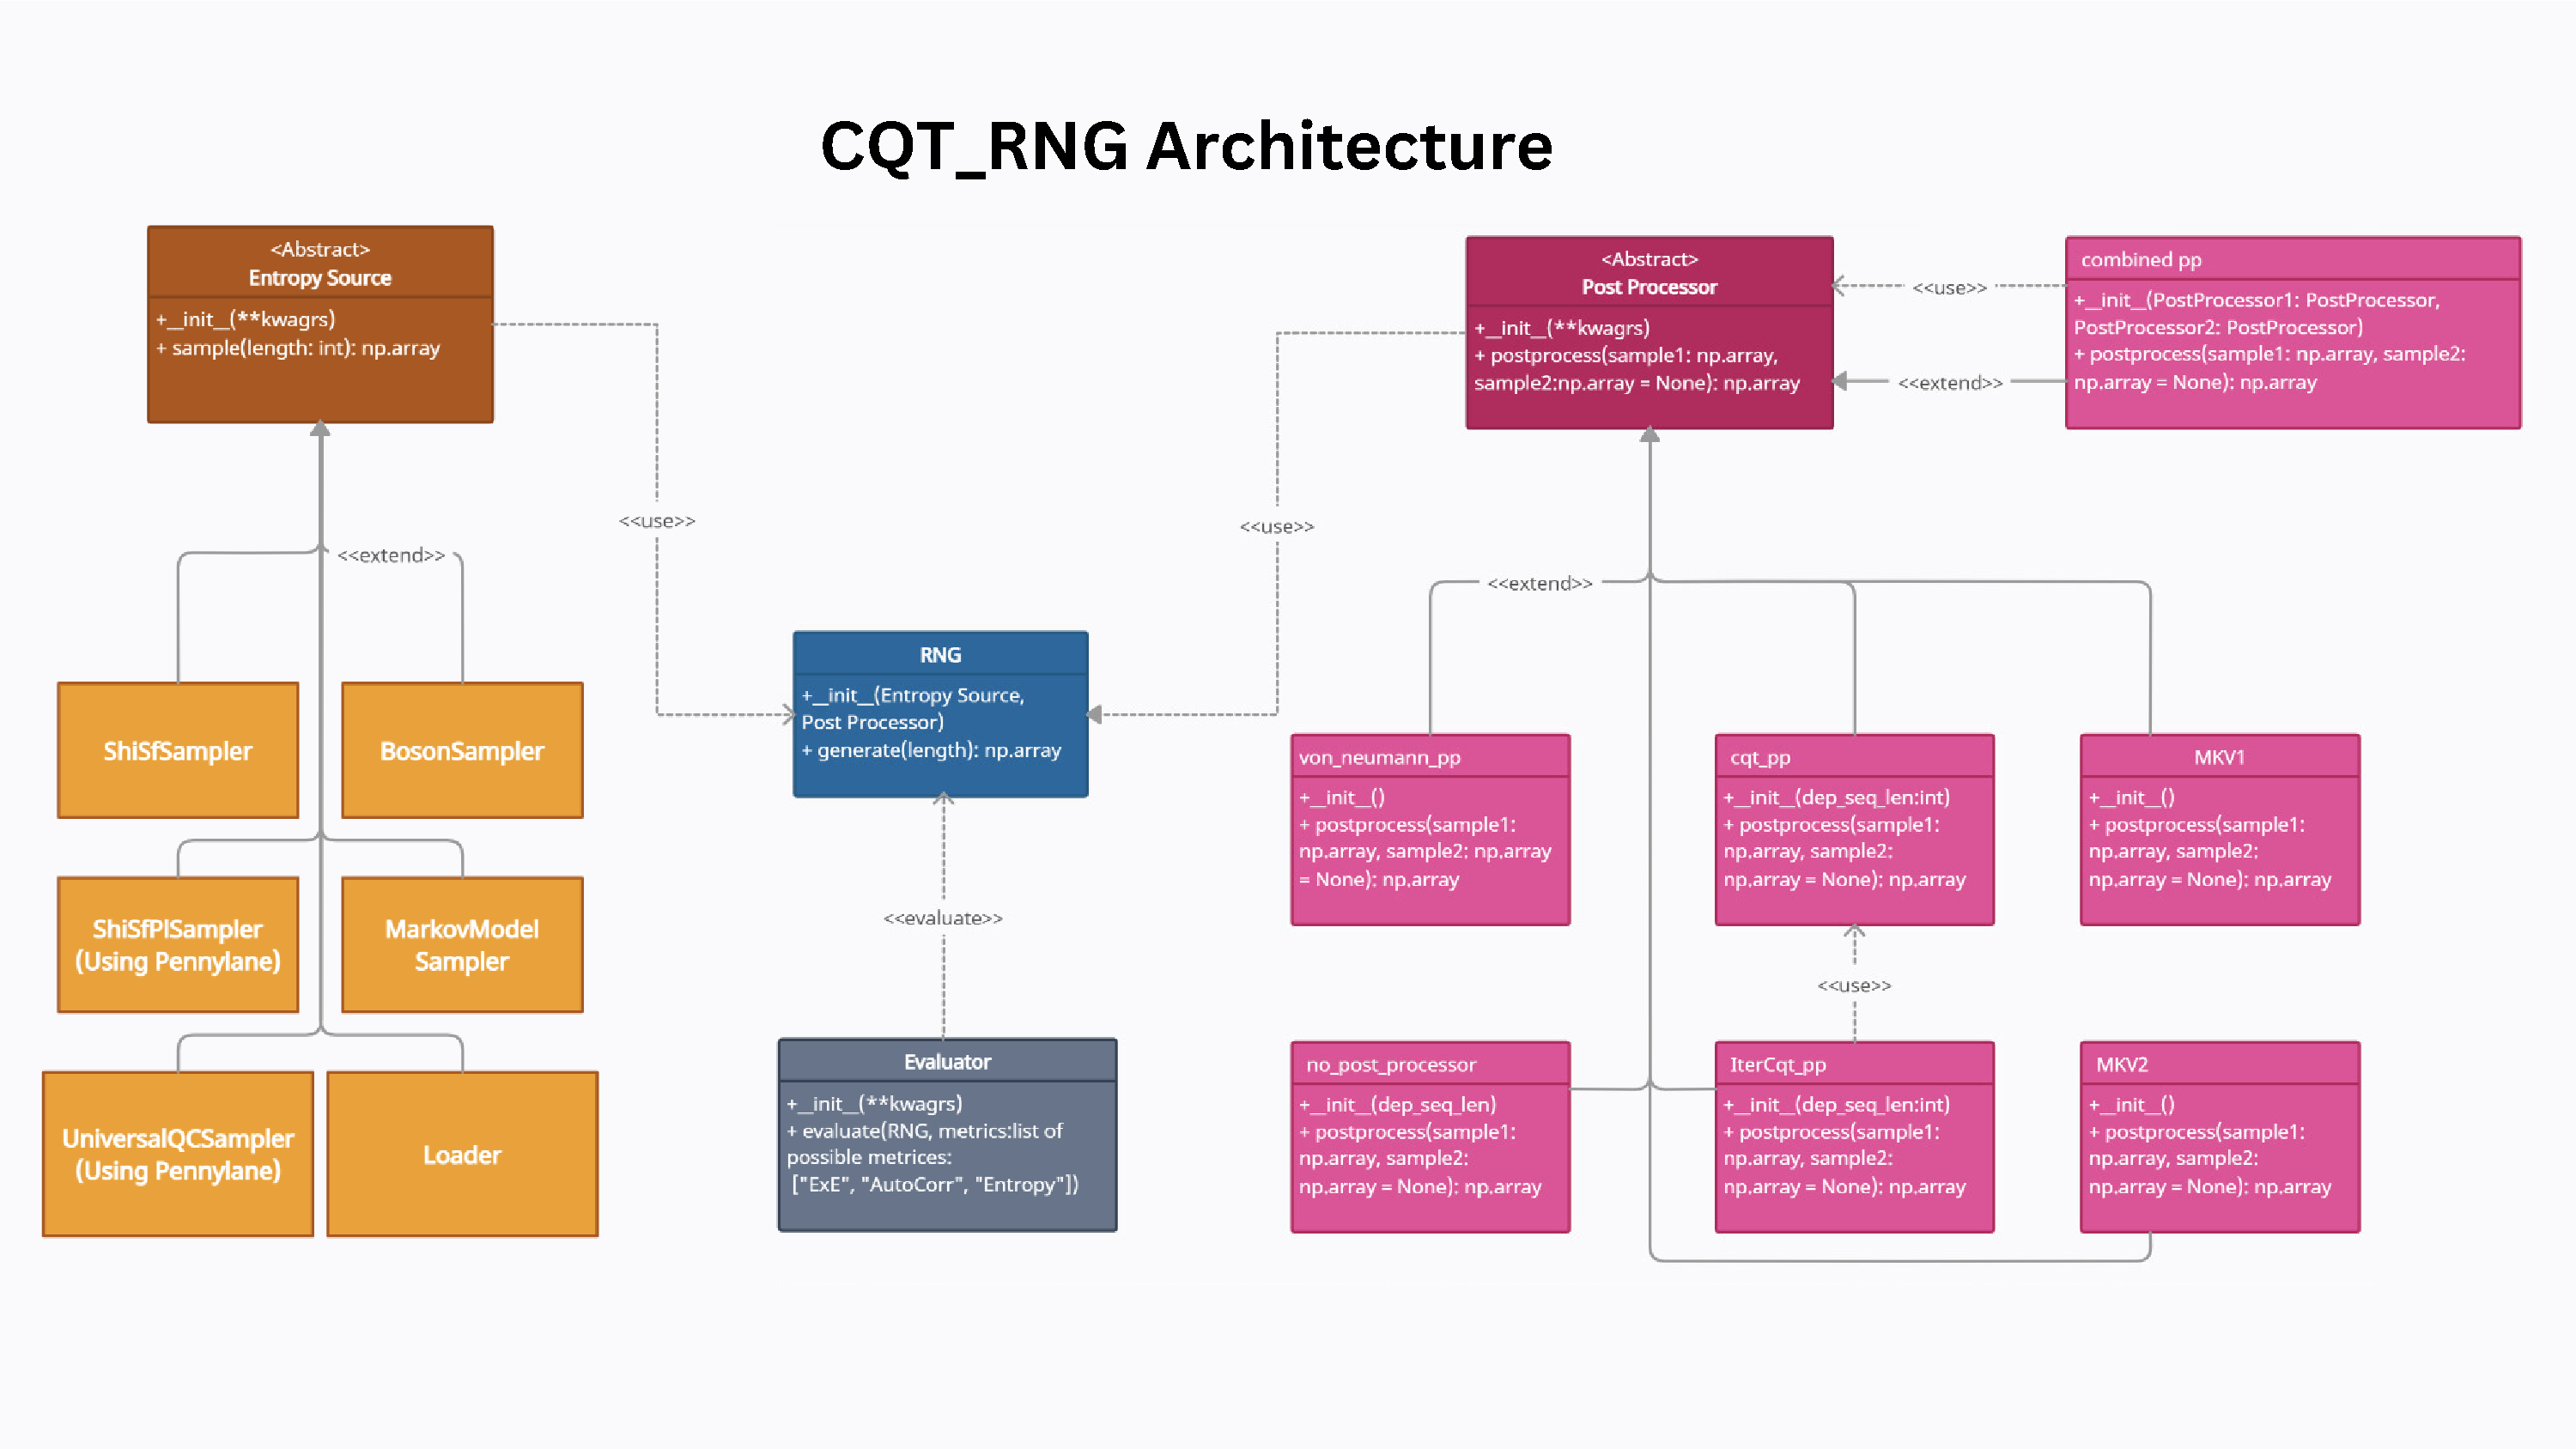
\includegraphics[width = 23cm]{figures/UML.pdf}
    \caption{The cqt\_rng2.0 architecture}
    \label{fig:UML}
\end{figure}
\end{landscape}
\section{This Study's Improvement on the Package: \texttt{cqt\_rng2.0}}

\subsection{Improvements}
\begin{enumerate}
    \item The post-processors can now process a single sample without the need to split it, while the two-sample mode still functions as intended.
    \item Fixed the two-sample length incoherence problem in the Von Neumann post-processor.
    \item Removed outdated modules causing installation errors in \texttt{cqt\_rng}, specifically the two real-device samplers (IBMQ and Borealis) which relied on deprecated packages, and the \texttt{UniversalQCSampler} which used an unsupported version of the IBM API.
    \item Fixed minor bugs and corrected conditional typos.
\end{enumerate}

\subsection{Introduced Novelties}
\begin{enumerate}
    \item Implemented the \texttt{ShiSampler} using Pennylane and a plugin for Strawberry Fields. This implementation was primarily for learning purposes, as writing photonic-based quantum circuits is not yet well-supported in Pennylane.
    \item Re-implemented the \texttt{UniversalQCSampler} using Pennylane, utilizing Hadamard and rotation gates to generate random data.
    \item Introduced the \texttt{Evaluator} module to assess RNG modules based on three functions:
    \begin{itemize}
        \item Extraction Efficiency
        \item Autocorrelation at lag \(k\)
        \item Shannon Entropy of \(n\)-bit words
    \end{itemize}
    \item Introduced the \texttt{MarkovSampler}, enabling the generation of bitlists with defined autocorrelation using the Markov model, which helps in evaluating RNGs.
    \item Added new post-processors such as \texttt{IterCQTPP} and Markov chains with 1-bit and 2-bit histories, as introduced in this study.
    \item Introduced the \texttt{CombinedPostProcessor}, which allows the chaining of two successive post-processors, such as \texttt{MKV+PostProcessor} and others.
    \item Added a new function in the \texttt{CQTPP} package that returns the discarded bits after applying the Von Neumann post-processor, enabling its use in \texttt{IterCQTPP}.
    \item Updated the setup and \texttt{\_\_init\_\_} files to include all required dependencies.
    \item Added the \texttt{generate\_markov\_model\_bitstring} function to the utilities module.
\end{enumerate}


\chapter{Conclusion} \label{ch6}
We revised some core Random Number Generation and True Random Number Generation principles to better understand the subject and have a hands-on approach to it, and then we discussed the three cornerstones that make a random number a truly random one. We have also discussed the actual pseudo RNGs and their reproducibility, as well as we gave an example in the appendices of how this problem can be used in the frame of the \textbf{seeds problem}. After that, we have seen how many researchers aimed to overcome these shortcomings by using physical systems (like \textbf{quantum ones}: those that interest us) that have noise as an entropy source and how these methods generate random numbers. Yet, they needed post-processing techniques to extract the uniform randomness we are looking for, and we saw how to evaluate the randomness using \textbf{autocorrelation} and \textbf{Shannon entropy}, as well as evaluating the \textbf{Extraction Efficiency} of the post-processors.

We discussed traditional post-processing techniques and their variants, such as the well-known \textbf{Von Neumann} method, the \textbf{Markov Chain de-correlator}, using the \textbf{Markov model}. We used it to generate some of our test data.

Then we moved on to discovering the main purposes of this study, which is to introduce the novel post-processing technique we named it \textbf{CQTPP} (\textbf{Constantine Quantum Technology Post Processor}) and some of the methods we tried to improve its throughput and compared it with the classical post-processors in order to try to overcome some of their defects, like the \textbf{Von Neumann method} that doesn't perform on inputs with dependencies.

We discussed the \textbf{boson sampling model} and how it is good as an \textbf{entropy source}.

We achieved that the \textbf{CQTPP} succeeded in matters of \textbf{badness} along with the \textbf{Von Neumann post-processor}. In the case of independent raw input, it is preferable to use the \textbf{VNPP} or one of its variants introduced in \cite{zonga}, since their rate can achieve \textbf{62.5\%} when using the \textbf{VN\_8 variant} and is much better than the classical \textbf{CQTPP} (around \textbf{17\%}) and its \textbf{Iter CQTPP}. However, if the input has correlations and has some dependency (\textbf{entanglement between bits}), it is much better to use the \textbf{CQTPP} with a \textbf{Markov chain de-correlator}, where results were near \textbf{0 autocorrelation}, unlike the \textbf{Von Neumann} method, which didn't change anything in terms of autocorrelation. The \textbf{Von Neumann + MKV} performs better but not as well as the \textbf{CQTPP + MKV}.

We also introduced the \textbf{CQT\_RNG2.0 package} and the improvements it contains and can be used and extended for study purposes.

This study aims to inspire and help individuals that don't have previous knowledge about the topic to get introduced to it, and as a trial to achieve better \textbf{decorrelation results} using the \textbf{CQTPost Processor}.

\label{chp-conclusion}




%% If your thesis has different "Parts", use commands such as the following:
%\part{First Part\label{part:one}}%
% \input{chap1}
%\input{chap2} % further chapters -- change file names to meaningful things...
%\input{chap3}
%\part{Second Part\label{part:two}}%
%\input{chap4}
%\input{chap5}
%\input{chap6}


%%%%% Appendices start %%%%%%%%%%%%%%%%
%% Comment out the following if your thesis has no appendix

\appendix

\chapter{Appendix}
%\section{Particle Image Velocimetry}
%\input{chapters/piv}

let's analyze the effectiveness of these results in terms of the nature of the input. We can review the results of most of the studies, as they considered the bits of the inputs were chosen independently.

\section{Classical VN with Independent Input}

Let's consider the input string \( x_1, x_2, \dots, x_i, \dots, x_m \) follows an independent distribution, where each \( x_i \) bit is chosen independently from the others and with a uniform bias (the probability of getting a 0 or 1 is fixed and not necessarily equal between them, but follows the same distribution).

Let the probability of \( x_i \) being 1 be \( p \), and the probability of \( x_i \) being 0 be \( q = 1 - p \), where \( p \) is unknown but satisfies \( 0 < p < 1 \).


Let's define the following set of events in terms of the output after post-processing a pair of bits:

\begin{enumerate}
    \item The generated output is a non-null output:
    \begin{itemize}
        \item The output is 0: The two input bits, according to the mapping, should be 01, where the first bit is 0 (with probability \( p \)) and the second bit is 1 (with probability \( q = 1 - p \)). Since these two events are independent, the probability for this output is
        \begin{equation}
        P(\text{Output is 0}) = p \cdot q = p \cdot (1 - p)
        \end{equation}
        \item The output is 1: The two input bits, according to the mapping, should be 10, where the first bit is 1 (with probability \( 1 - p \)) and the second bit is 0 (with probability \( p \)). Since these two events are independent, the probability for this output is
        \begin{equation}
        P(\text{Output is 1}) = q \cdot p = (1 - p) \cdot p = p \cdot (1 - p)
        \end{equation}
    \end{itemize}
    Thus, to generate a non-null output:
    \begin{equation}
    P(\text{Output is not null}) = P(\text{Output is 0}) + P(\text{Output is 1}) = 2p(1 - p)
    \end{equation}

    \item The generated output is a null output (the pair is discarded):  
    This event can be easily defined as:
    \begin{equation}
    P(\text{Output is null}) = 1 - P(\text{Output is not null})
    \end{equation}
\end{enumerate}


Thus, to generate a non-null output:
\begin{equation}
P(\text{Output is not null}) = P(\text{Output is 0}) + P(\text{Output is 1}) = 2p(1 - p)
\end{equation}

In order to deduce that the output is unbiased, we need to confirm that the probability of having 0 in the output is the same as the probability of having 1.

From the events described above, we have 
\begin{equation}
P(\text{Output is 1}) = p(1-p) = k \quad \text{and} \quad P(\text{Output is 0}) = p(1-p) = k
\end{equation}
Thus,
\begin{equation}
P(\text{Output is 1}) = P(\text{Output is 0}) = k
\end{equation}
where \( 0 < k < 1 \). Therefore, the probability of having 0 in the output is the same as the probability of having 1, which allows us to conclude that the results of the classical Von Neumann post-processing with independent and uniformly biased input are unbiased.

\section{Classical VN with Dependent Input}

First, let's define an input with dependent elements. A bitstring can be considered dependent when the probability of a bit being either \( 0 \) or \( 1 \) relies on the bit before it. We can model this dependency using conditional probabilities as follows:  

1. **The \( x_{i+1} \) bit is the same as the \( x_i \):**  
   \begin{equation}
   P(x_{i+1} = x_i) = P(x_{i+1} = 0 \,|\, x_i = 0) = P(x_{i+1} = 1 \,|\, x_i = 1) = \lambda
   \end{equation}  

2. **The \( x_{i+1} \) bit is the inverse of the previous bit:**  
   \begin{equation}
   P(x_{i+1} \neq x_i) = P(x_{i+1} = 0 \,|\, x_i = 1) = P(x_{i+1} = 1 \,|\, x_i = 0) = 1 - \lambda
   \end{equation}  

Here, \( \lambda \) represents the degree of correlation, and \( \lambda \neq 0.5 \) (dependent case).  

If we follow the same pattern as we did with independent elements to prove the unbiasedness of the results of the Von Neumann post-processing method, let’s redefine the previous set of events, assuming that each bit can be \( 0 \) with probability \( p \) and \( 1 \) with probability \( q = 1 - p \). \\ 


\noindent So To generate a non-null output: \\ 

1. \textbf{The output of the post-processor is \( 0 \):}  
The input pair of bits should be \( 01 \). Using the formula for conditional probability:  
   \begin{equation}
   P(\text{Output} = 0) = P(x_i = 0 \cap x_{i+1} = 1) = P(x_{i+1} = 1 \,|\, x_i = 0) \cdot P(x_i = 0)
   \end{equation}  
   Substituting from the correlation model:  
   \(
   P(x_{i+1} = 1 \,|\, x_i = 0) = 1 - \lambda
   \)
   So:  
   \begin{equation}
   P(\text{Output} = 0) = (1 - \lambda) \cdot p \dots (1)
   \end{equation}  

2. \textbf{The output of the post-processor is \( 1 \):}
   The input pair of bits should be \( 10 \). The probability of the first bit being \( 1 \) is \( q = 1 - p \), and the second bit being \( 0 \) is \( P(x_{i+1} = 0 \,|\, x_i = 1) \). Using the same formula:  
   \begin{equation}
   P(\text{Output} = 1) = P(x_i = 1 \cap x_{i+1} = 0) = P(x_{i+1} = 0 \,|\, x_i = 1) \cdot P(x_i = 1)
   \end{equation}  
   Substituting from the correlation model:  
   \(
   P(x_{i+1} = 0 \,|\, x_i = 1) = 1 - \lambda
   \)  
   So:  
   \begin{equation}
   P(\text{Output} = 1) = (1-\lambda) \cdot (1 - p) = (1-\lambda) \cdot q  \dots (2)
   \end{equation}
   


   For the output to be unbiased, the probabilities of \( 0 \) and \( 1 \) must be equal:  
   \begin{equation}
   P(\text{Output} = 0) = P(\text{Output} = 1)
   \end{equation}  
   Substituting from \( (1)  and  (2): \) 
   \begin{equation}
   (1 - \lambda) \cdot p = (1-\lambda) \cdot (1 - p)
   \end{equation}  
   Simplifying:  
   \begin{equation}
   (1- \lambda) \cdot (2p-1) = 0
   \end{equation}  
   
   So:  
   \[
   p = 0.5
   \]  

For the Von Neumann Post-Processor to produce unbiased results, the input must be uniformly distributed and unbiased. However, this contradicts the initial assumption of the input being dependent and uniformly biased as outlined in the study. Therefore, with dependent input, the output of the Von Neumann Post-Processor is \textbf{biased}.

\section{Codes and algoirthms}



% Include all pages from your PDF file
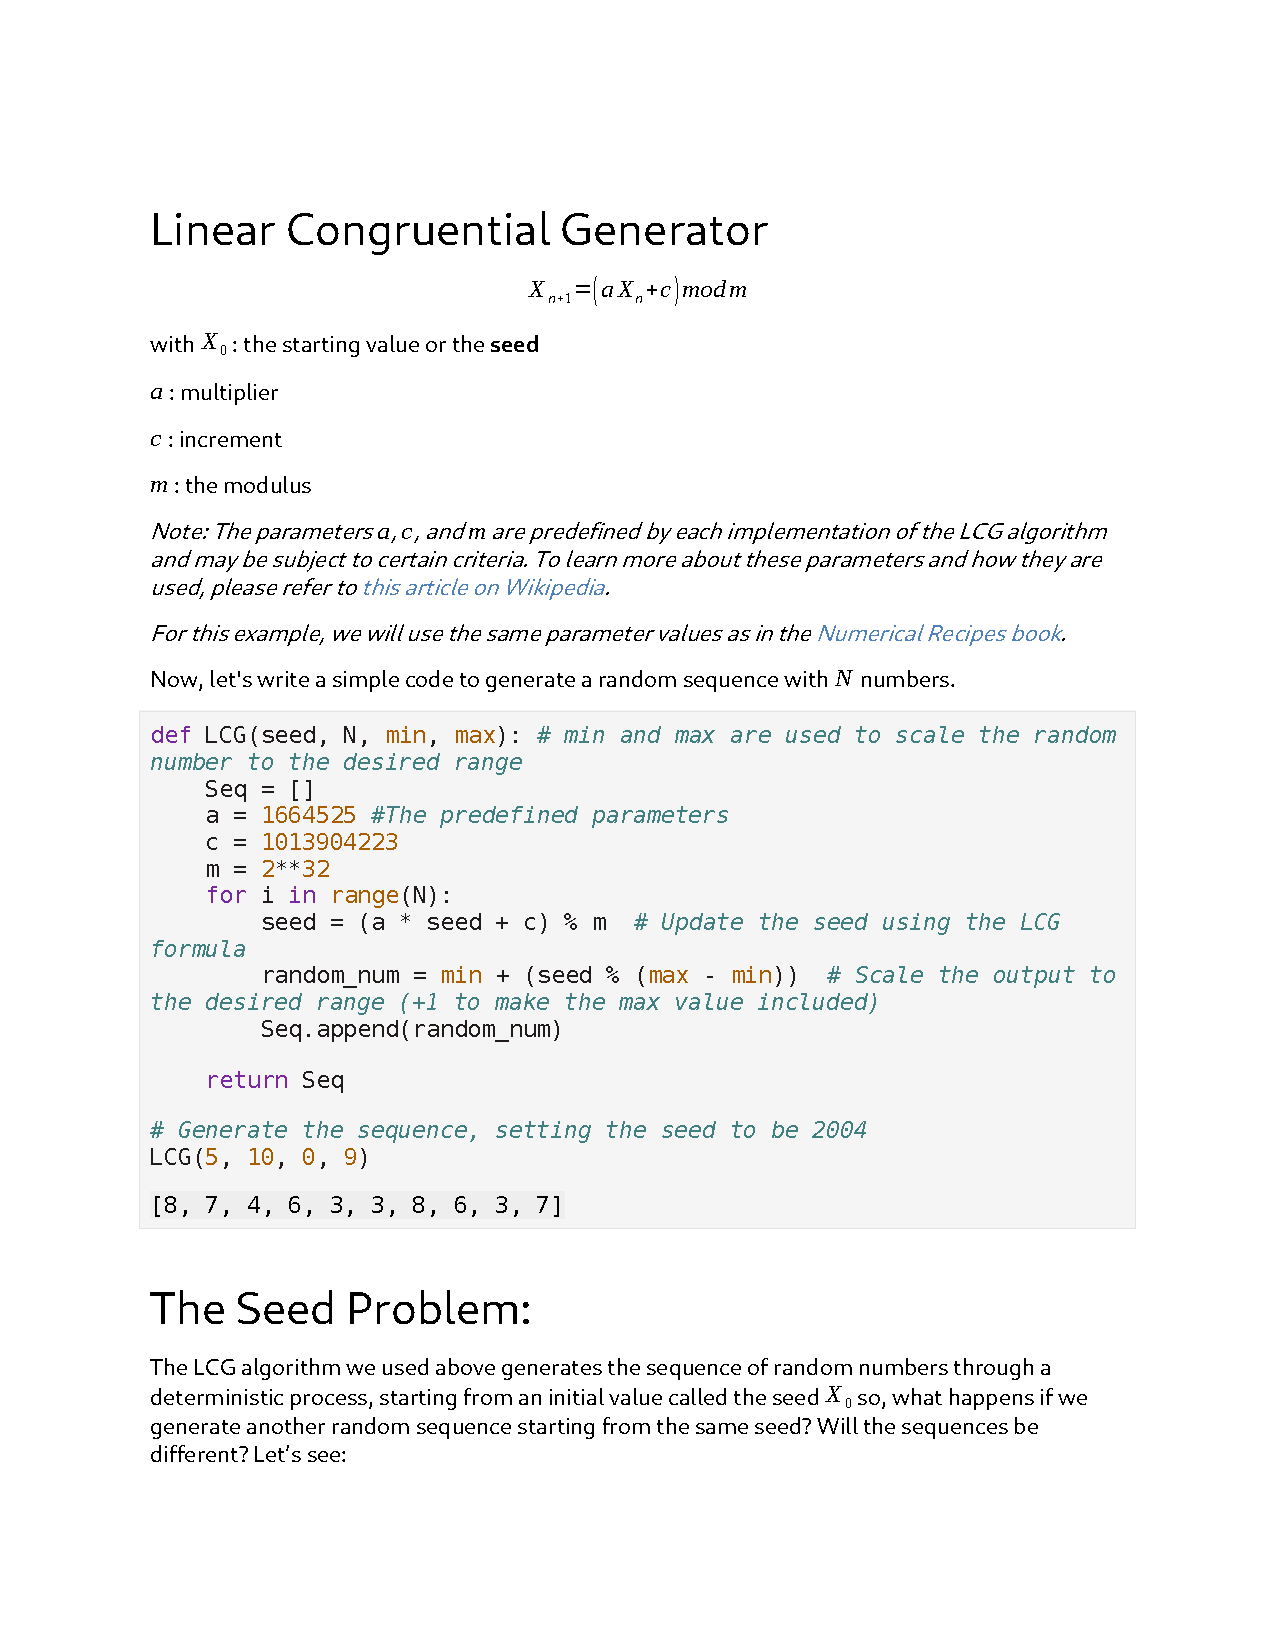
\includepdf[pages=-]{chapters/vertopal.com_QRNG Ashraf Appendix.pdf}




%% Note: If your thesis has more than one appendix, NYU requires a "list of
%% appendices" page before the body of the thesis. I don't provide the tools
%% to create that here, so you're on your own for that one... Sorry.


%%%% Input bibliography file %%%%%%%%%%%%%%%
%% For computer science dissertations, I'd recommend using the bibly package
%% to automatically create the .bib file from your citations:
%% https://github.com/michael-emmi/bibly

\cleardoublepage
\phantomsection

%\bibliographystyle{plainnat}
%\RequirePackage{doi}
%\bibliographystyle{apalike}
%\bibliographystyle{abbrv}
\addcontentsline{toc}{chapter}{References}

 %\nocite{*}
\printbibliography
\end{document}

%%% Local Variables:
%%% mode: latex
%%% TeX-master: t
%%% End:
